\graphicspath{{./02figs/}}

%\tableofcontents

\chapter{Methods}
Collision events are characterised by a 
range of dynamical 

%\subsection*{Introduction}
%\includepdf[pages={2-},fitpaper=true]{/tree_musings}

Motivation to use SPH, spatial dynamics of collisions, SPH particles are where the mass is (not entirely true for collisions, but necessary), free boundaries



Lagrangian nature vs. grid techniques, complexity of AMR vs. simplicity of SPH

Neighbour search is the hardest thing about SPH



In this chapter we will discuss, how collisions in the strengthless regime as appearing in planetary systems can be modelled.
The first section gives a short review the governing physics of such collisions and will provide us with a closed set of equations, namely the Navier-Stokes equations and the 
This set is far too complicated to be solved in an analytical way. 
Smoothed particle Hydrodynamics (SPH) is a method which discretises fluids with particles of finite volume and presents a framework to solve the equations describing the fluid.
The second section derives different SPH formulations of the Navier-Stokes equations and demonstrates the advantages and disadvantages of each formulation.

gravity section: 

The initial conditions and also the outcome of collisional events can be charaterized by a 

Smoothed particle hydrodynamics (SPH) is a numerical method which can discretize 

(insert a nice picture of equations, code lines and numbers here)

\newpage

\section{Fluid- and Thermodynamics}
A continuum model 

%%
%   F L U I D S
%%
\subsection{Fluids}
A fluid is a classical continuum approximation of an ensemble of molecules or atoms. Characteristic variables defined continuously are density $\rho$, specific internal energy $u$, temperatur $T$, velocity $\vv$ and pressure $p$. Conservation of mass leeds directly to the continuum equation, which equals the local change density to the negative product of velocity divergence and density:
\begin{equation}
\label{ch02_fld01_eq001}
\frac{\partial \rho}{\partial t} + \rho \nabla \mathbf{v} = 0
\end{equation}

Momentum conservation ultimately gives us the \emph{Navier-Stokes equation} 
\begin{equation}
\label{ch02_fld01_eq002}
\rho \frac{\partial \mathbf{v}}{\partial t} + \rho ( \mathbf{v} \nabla ) \mathbf{v} = - \nabla p + \nabla \Phi + \nu \Big( \nabla^2 \vv - \frac{2}{3} \nabla \nabla \vv \Big)
\end{equation}

for a viscous fluid, where $\nu$ is the kinematic viscosity and $\Phi$ any external potentials acting on the fluid like gravity \citep{shore2007astrophysical}. In the absence of viscosity and external potentials, the equation reduces  to the momentum equation of the \emph{Euler equations}

\label{ch02_fld01_eq003}
\begin{equation}
- \frac{\partial \mathbf{v}}{\partial t} =  ( \mathbf{v} \nabla ) \mathbf{v} + \frac{\nabla p}{\rho}
\end{equation}

Energy conservation in the absence of dissipative terms (constant entropy) yields
\label{ch02_fld01_eq003a}
\begin{equation}
\frac{\d}{\d t} \Big( \rho u + \frac{1}{2}\rho \vv^2 \Big) + \nabla \vv\Big( \rho u + \frac{1}{2} \rho \vv^2 + p \Big) = 0
\end{equation}

Those equations are formulated in an eulerian frame a rest. If we choose a frame of reference at rest relative to the fluid, we get a Lagrangian description of the momentum equation \ref{ch02_fld01_eq003} where the advection term $\vv (\nabla \vv)$ vanishes:

\begin{equation}
\label{ch02_fld01_eq003b}
- \frac{\partial \mathbf{v}}{\partial t} = \frac{\nabla p}{\rho}
\end{equation}

The continuity equation is un-affected by the choice of a Lagrangian frame of reference, as it depends only on the velocity divergence and not the absolute velocity. The actual Lagrangian of a in-viscous fluid without an external potential is given by
\begin{equation}
\label{ch02_fld01_eq004}
\Lagr = \int \Big( \frac{1}{2} \rho \vv ^2 - \rho u \Big) dV
\end{equation}

%%
%   S P H
%%
\subsection{SPH formalism}
The basic idea of SPH is to interpolate all continuum variables in space with an interpolant.
If our variable is $A(\rv)$ defined at all points in space $\rv$, we start with the basic equality

\begin{equation}
\label{ch02_sph01_eq001}
A(\rv) = \int  \delta(\rv - \rvs) A(\rvs) \ud \rvs
\end{equation}

We now replace the $\delta$-function with a smoothing kernel $W$, which has typical width $h$, the smoothing length, and which fulfils the following two criteria

\begin{equation}
\label{ch02_sph01_eq002}
\limhzero W(\rv - \rvs, h) = \delta(\rv - \rvs) \hspace{1.0cm}
\int W(\rv - \rvs, h) \ud \rvs = 1
\end{equation}

Equation \ref{ch02_sph01_eq001} can now be re-written as 

\begin{equation}
\label{ch02_sph01_eq003}
A(\rv) = \int  W(\rv - \rvs, h) A(\rvs) \ud \rvs + O(h^2)
\end{equation}

The variable $A(\rv)$ is now smoothed out over the characteristic scale $h$. By replacing the $delta$-function with a kernel of finite length, an error in the order of $h^2$ is introduced. Now comes the particle part: The continuum is replaced by a finite set of points (\emph{particles}), on which the quantities are defined. The integral can now be replaced by a sum with a finite number of summands:

\begin{equation}
\label{ch02_sph01_eq004}
A(\rv) \approx \sum_{j} W(\rv - \rvj) A_i V_{j} \hspace{1.0cm} V_{j} = \frac{m_j}{\rho_j}
\end{equation}

$V_{j}$ is the particle volume and is usually given assigning each particle a mass and dividing it by the density. The particles used in the summation are called \emph{neighbours} and are indexed here with $j$. For most purposes, the variable only needs to be known at particle position $i$. For convenience, we write the kernel used between two particles as $\Wij = W( \rvi - \rvj, h)$

If the smoothing length goes to zero and the number of neighbours goes to infinity, the sum \ref{ch02_sph01_eq004} approximates the integral \ref{ch02_sph01_eq001} exactly. This is the \emph{SPH limit}.

Spatial derivatives are easily given by taking the partial derivative of the integral interpolant variable and replacing it again by the sum over all neighbours:

\begin{equation}
\label{ch02_sph01_eq005}
\nabla A(\rv_i) = \frac{\partial}{\partial \rv}\int A(\rvs) \ud \rvs \frac{\partial}{\partial \rv}\ W(\rv_i - \rvs, h) + O(h^2)
\approx \sum_{j} A_j V_{j} \nabla \Wij 
\end{equation}

Rotations of variables can be similarly obtained:
\begin{equation}
\label{ch02_sph01_eq006}
\nabla \times A_i \approx \sum_{j} A_i V_{j} (\nabla \times \Wij)
\end{equation}

Like in in grid based schemes, there are different ways of calculating spatial derivatives in SPH.
Depending on the actual application of the derivative, whether it is to get the velocity divergence or a pressure gradient, there are better suited variants which show better error behaviour. They will be presented shortly.

The kernel has to fulfill the two constraints posed by equations \ref{ch02_sph01_eq002}. A natural choice would be a normalized Gaussian, but this has the unpleasant of never vanishing. All particles, also distant ones, would contribute to every individual SPH sum, making the method very inefficient. A better choice are therefore functions with compact support: Functions which vanish at sufficiently large distances. A common selection are cubic splines

\begin{equation}
\label{ch02_sph01_eq007}
W(| \rv |, h) = \frac{\sigma}{h^\nu \pi} \left \{ \begin{array}{lll}
1 - \frac{3}{2}q^2 + \frac{3}{4}q^3 & r \leq h & \\
\frac{1}{4}(2-q)^3 & h < r  \leq 2h & \hspace{1.0cm} q = r / h\\
0 & 2h < r & \\
\end{array} \right. 
\end{equation}

where $\nu$ stands for the number of spatial dimensions and $\sigma = \big( \frac{2}{3}, \frac{10}{7\pi}, \frac{1}{\pi} \big) $ for $\big( 1,2,3\big)$ dimensions. The Kernel vanishes for distances greater than $2h$, reducing SPH sums to contributing terms of only the nearest neighbours. The first derivative is given by 

\begin{equation}
\label{ch02_sph01_eq008}
\nabla W(\rv, h) = \frac{\rv}{r} \frac{\sigma}{h^\nu \pi} \left \{ \begin{array}{ll}
1 - 3q + \frac{9}{4}q^2 & r \leq h \\
\frac{3}{4}(2-q)^2 & h < r  \leq 2h \\
0 & 2h < r \\
\end{array} \right. 
\end{equation}

and is also continuous. 

The choice of the smoothing length is a trade-off. It is large compared compared to the spacing between the particles, then the variables are smoothed out over too large distances and small features cannot be resolved. If the smoothing length is too small, the variables are not sufficiently smoothed and get very noise, ultimately leading to instabilities. As a golden rule, the smoothing length should be chosen, such as the number of neighbors is 50 inside a radius of $2h$. For a hexagonal HCP lattice in 3D with a lattice constant $k$, this leads to $h \approx 0.85 k$. 

\subsection{standard SPH}
The original and most widely used version of SPH uses the density and particle mass to calculate the particle volumes ($V_j = m_j / \rho_j)$ and the density to interpolate all variables. The density is given by the simple particle sum

\begin{equation}
\label{ch02_sph02_eq001}
\rho_i = \sum_{j} m_j \Wij
\end{equation}

The velocity divergence $\nabla \vv$ could in principle be written as
\begin{equation}
\label{ch02_sph02_eq002}
\nabla \vv_i = \sum_{j} \frac{m_j}{\rho_j} \vv_j \nabla \Wij
\end{equation}

but this form has the disadvantage of being asymmetric and will ultimately lead to a non-conservative form for the linear momentum. It is better to apply the \emph{second golden rule} of SPH \citep{Monaghan:1992p3721} to re-write the velocity divergence term with the density placed inside the operators:

\begin{equation}
\label{ch02_sph02_eq003}
\nabla \vv = \frac{1}{\rho} \Big( \nabla (\rho \vv) - \vv \nabla \rho \Big)
\end{equation}

so that the corresponding SPH sum becomes 

\begin{equation}
\label{ch02_sph02_eq003}
\nabla \vv_i = \frac{1}{\rho_i} \sum_{j} \frac{m_j}{\rho_j} \rho_j \vv_j \dWij - \frac{1}{\rho_i} \vv_i \sum_{j} \frac{m_j}{\rho_j} \rho_j \dWij = \frac{1}{\rho_i} \sum_{j} m_j \vvij \dWij 
\end{equation}

with $\vvij = \vv_j - \vv_i$, which is a symmetric form for the velocity divergence. If we take the partial time derivative of \ref{ch02_sph02_eq001}, where only the particle positions in the Kernel depend explicitly on time, we get: 

\begin{equation}
\label{ch02_sph02_eq004}
\frac{\partial \rho_i}{\partial t}  = \sum_{j} m_j \Big( \frac{\partial}{\partial t} \rvij \Big) \nabla \Wij = \sum_{j} m_j \vvij \nabla \Wij 
\end{equation}

So this equation together with the velocity divergence equation \ref{ch02_sph02_eq003} fulfills the continuity equation \ref{ch02_fld01_eq001} for each particle.

The equations of motion can be derived in two different ways: With the inviscous equation of motion of the Navier-Stokes equation \ref{ch02_fld01_eq003}, a symmetric formulation for the pressure gradient term $\nabla p / \rho$ can be found with the trick used above for the velocity divergence. 
A more elegant way is to derive the equation of motion directly from the Lagrangian given by equation \ref{ch02_fld01_eq004}, whose SPH formulation is

\begin{equation}
\label{ch02_sph02_eq004}
\Lagr = \sum_{j} m_j \Big( \frac{1}{2} \vv_j^2 - u(\rho_j, s_j) \Big) 
\end{equation}

where $u$ is the specific internal energy of a fluid particle dependent only on its density and specific entropy $s$. The Euler-Lagrange equations for a single particle $i$ is

\begin{equation}
\label{ch02_sph02_eq005}
\frac{d}{dt} \Big( \frac{\partial \Lagr}{\partial \vv_i} \Big) - \frac{\partial \Lagr}{\partial \rv_i} = 0
\end{equation}

which yields 

\begin{equation}
\label{ch02_sph02_eq006}
m_i \frac{d \vv_i }{dt} = \sum_{j} m_j \frac{\partial u_j}{\partial \rho_j} \frac{\partial \rho_j}{\partial \rv_i}
\end{equation}

for constant entropy, which is the case in the absence of shocks. The first law of thermodynamics for a particle is given by

\begin{equation}
\label{ch02_sph02_eq007}
\frac{u_j}{\rho_j} = \frac{p_j}{\rho_j^2}
\end{equation}

and the divergence of the density is directly given by

\begin{equation}
\label{ch02_sph02_eq008}
\frac{\partial }{\partial \rv_i} \rho_j
= \sum_{k} m_k \frac{\partial}{\rv_i} W_{jk} 
= \sum_{k} m_k \nabla W_{jk} ( \delta_{ji} - \delta_{ki})
\end{equation}

where the kernel vanishes except if $i = j$ and if $i = k$. So equation \ref{ch02_sph02_eq006} yields

\begin{equation}
\label{ch02_sph02_eq009}
m_i \frac{d \vv_i }{dt} = \sum_{j} m_j \frac{p_j}{\rho_j^2} \sum_{k} \nabla_i W_{jk} ( \delta_{ji} - \delta_{ki})\\
 = m_i \sum_{j} m_j \Big( \frac{p_i}{\rho_i^2} + \frac{p_j}{\rho_j^2} \Big) \nabla W_{ij}
\end{equation}

and leaves us with a symmetric SPH sum for the acceleration of a particle in absence of shocks:
\begin{equation}
\label{ch02_sph02_eq010}
\frac{d \vv_i }{dt} = \sum_{j} m_j \Big( \frac{p_i}{\rho_i^2} + \frac{p_j}{\rho_j^2} \Big) \nabla W_{ij}
\end{equation}

The derivative of the kernel is anti-symmetric ($\nabla W_{ij} = - \nabla W_{jj}$), therefore each interacting particle pair fulfils Newtons third law \emph{actio-reactio} and linear momentum is conserved. Angular momentum is also conserved, which can be shown by taking the time derivative of the $\frac{d}{dt} \sum_i (m_i \rv_i \times \vv_i)$ where some index magic \citep{Price:2004p2613} again shows that all terms cancel each other out in the sum over all particles.

In most cases, the internal enery of the fluid is non-constant, so we also need a equation for the change in internal energy due to compressional heating.
The rate of change in specific internal energy is given by 

\begin{equation}
\label{ch02_sph02_eq011}
\frac{du}{dt} = -\frac{p}{\rho} \nabla \vv
\end{equation}

Using the velocity divergence SPH sum \ref{ch02_sph02_eq003}  yields

\begin{equation}
\label{ch02_sph02_eq012}
\frac{du_i}{dt} = \frac{p_i}{\rho_i^2} \sum_{j} m_j \vvij  \dWij
\end{equation}

An SPH sum of this equation consistent with the equation of motion from above can be obtained by applying the golden rule again and putting the density inside the divergence operators:

\begin{equation}
\label{ch02_sph02_eq013}
\frac{du}{dt} = - \nabla \Big( \frac{p \vv}{\rho} \Big) + \vv \nabla \Big( \frac{p}{\rho} \Big)
\end{equation}

The corresponding SPH sum yields the asymmetric equation

\begin{equation}
\label{ch02_sph02_eq014}
\frac{du_i}{dt} = - \sum_{j} m_{j} \frac{p_j \vv_j}{\rho_j} \dWij + \vv_i \sum_{j} m_{j} \frac{p_j}{\rho_j^2}  \dWij = \sum_{j} m_j \vvij \frac{p_j}{\rho_j^2}  \dWij
\end{equation}

A symmetric formulation can be gained by taking the average of equations \ref{ch02_sph02_eq012} and \ref{ch02_sph02_eq014}:

\begin{equation}
\label{ch02_sph02_eq015}
\frac{du_i}{dt} = \frac{1}{2} \sum_{j} m_{j} \vvij \Big( \frac{p_i}{\rho_i^2}  + \frac{p_j}{\rho_j^2} \Big) \dWij
\end{equation}

\subsection{Resolving shocks}
Shocks are changes of the characteristics of a fluid on the spatial scale of the molecules mean-free path. Discontinuities arise in the fluid approximation, usually in density, pressure and temperature.
Numerical schemes tend to react to these discontinuities with unphysical oscillations behind the shock front, because the sharp changes cannot be resolved properly.
Several approaches exist to tackle this problem. Godunov-schemes solve the Riemann problems on both sides of the shock exactly between computational elements and in a second step superpose all pair-wise solutions for each element. In case of SPH this can be done by solving the Riemann problem for each particle against its neighbours \citep{Monaghan:1997p3938}.
Another approach is the von Neumann and Richtmyer viscosity: By introducing a small amount of viscosity, the \emph{artificial viscosity}, the shock front is smoothed out and the oscillations disappear. This can be implemented in SPH by adding additional terms to the momentum and energy equation. The most common used variant is that given by \citep{Monaghan:1992ARAA..30..543M}:

\begin{equation}
\label{ch02_sph02_eq016}
\frac{d \vv_i }{dt} \Big|_{AV} = \sum_{j} m_j \frac{-\alpha c_{ij} \mu_{ij} + \beta \mu_{ij}^2}{\rho_{ij}} \dWij \hspace{1.0cm} \mu_{ij} = \frac{h \vvij \rvij}{\rvij^2 + 0.01h^2}  \hspace{0.5cm} \mathrm{if}  \hspace{0.5cm} \rvij \vvij < 0
\end{equation}

where $\rho_{ij}$ is the averaged density between two particles and $\mu_{ij}$ is a signal velocity with an order of magnitude of the speed of sound. The artificial viscosity term is only applied in situations of compression, where $\rvij \vvij < 0$. The choice of constants is usually $\alpha = 1$ and $\beta = 2 \alpha$. The $\beta$-term is the actual von Neumann and Richtmyer term and becomes dominant in strong shocks where the velocity difference $\vvij$ between two particles in the shock front becomes large. Momentum conservation is still conserved by the symmetric form of the artificial viscosity term.

The contribution of artificial viscosity to the internal energy can be found by requiring that artificial viscosity itself should be energy conserving. The specific energy change due to the dissipative is given by

\begin{equation}
\label{ch02_sph02_eq017}
\frac{de_i}{dt} \Big|_{AV}  = \frac{du_i}{dt}  \Big|_{AV} + \vv_i \frac{d\vv_i}{dt}  \Big|_{AV} = 0
\end{equation}

and should be zero. This leads to the thermal contribution

\begin{equation}
\label{ch02_sph02_eq018}
\frac{du_i }{dt} \Big|_{AV} = - \sum_{j} m_j \vvij \frac{-\alpha c_{ij} \mu_{ij} + \beta \mu_{ij}^2}{\rho_{ij}} \dWij
\end{equation}

with the same choice for the signal velocity $\mu_{ij}$ and numerical constants as in equation \ref{ch02_sph02_eq016}. 

A disadvantage of this approach is that this viscosity also acts outside of shocks in situations of weak compression or shear flows. There exist several approaches to fix this issue by detecting shocks more cleverly \citep{Morris1997J.-Comput.-Phys.Morris} than the simply checking for compression or recognizing shear flows explicitly \citep{Balsara1995JCoPh.121..357B} and suppressing the artificial viscosity in situations where it is not needed. For the simulation of collisions, this is not a big problem, therefore we don't include such fixes.

\subsection{variable smoothing length}
In order to meet the requirement of $50$ neighbors per particle, the smoothing is adjusted for each particle individually. For constant particle masses the density is proportional to the particle density $\delta_i$, which again is inverse proportional to the particle volume and therefore to the inverse third power of the smoothing length in 3D:

\begin{equation}
\label{ch02_sph02_eq026}
\rho_i \sim \delta_i \sim \frac{1}{V_i} \sim \frac{1}{h_i^3}
\end{equation}

So the rate of change of the smoothing length is given by using the continuity equation \ref{ch02_sph02_eq005} yields

\begin{equation}
\label{ch02_sph02_eq027}
\frac{d h_i}{dt} = - \frac{h_i}{3 \rho_i} \frac{d \rho_i}{dt} = \frac{1}{3} h_i \nabla \vv_i
\end{equation}

This keeps the number of neighbours exactly constant, if the particle density changes isotropically. Usually this is not the case and the number of neighbors ($N_N$) becomes either too large or too small. In such cases it is useful to overcorrect the smoothing length with the global maximum of velocity divergence ($\nabla \vv_{max} = \max_{i} \nabla \vv_i$):

\begin{equation}
\label{ch02_sph01_eq028}
\frac{d h_i}{d t} = h_i ( k_1 \nabla \vv_{max}+ k_2 \frac{1}{3} \nabla\vv_i - k_3 \nabla \vv_{max} )
\end{equation}

\begin{equation}
\label{ch02_sph01_eq029}
\begin{array}{ll}
k_1 = \frac{1}{2} (1 + \tanh{- \frac{N_N - N_{N,min}}{5}} ) & N_{N,min} = \frac{2}{3} N_{N,opt} \\
k_2 = 1 - k_1 - k_3 & \\
k_3 = \frac{1}{2} (1 + \tanh{\frac{N_N - N_{N,max}}{5}} ) & N_{N,max} = \frac{5}{3} N_{N,opt}\\
\end{array}
\end{equation}

If the number of neighbours is within $\frac{2}{3} N_N$ and $\frac{5}{3} N_N$, the expression \ref{ch02_sph02_eq027} is dominant. If it's below or above the optimal number, the change rate of the smooting length is over- or under-corrected with the maximum velocity divergence. In practice, this scheme keeps the number of neighbors in reasonable limits, without introducing any instabilities.

\subsection{Integration}
Together with an equation of state which gives us the pressure $p_i(u_i, \rho_i)$ and as a side effect also the speed of sound $c_i(u_i, \rho_i)$, we have a closed set of equations describing the fluid which can be integrated in time. A common choice due to its simplicity and low number of derivation steps required is the predictor-corrector scheme \citep{Press2002nrc..book.....P}. For the integration of particle positions we use the second-order form, which yields the prediction step

\begin{eqnarray}
\label{ch02_sph02_eq019}
\rv_i^{(p)} = \rv_i^{(0)} + \frac{1}{2} ( 3 \vv_i^{(0)} - \vv_i^{(-1)} )\Delta t \\
\vv_i^{(p)} = \vv_i^{(0)} + \frac{1}{2} ( 3 \av_i^{(0)} - \av_i^{(-1)} )\Delta t
\end{eqnarray}
and the correction step

\begin{eqnarray}
\label{ch02_sph02_eq020}
\rv_i^{(1)} = \rv_i^{(0)} + \frac{1}{2} ( \vv_i^{(p)} - \vv_i^{(0)} )\Delta t \\
\vv_i^{(1)} = \vv_i^{(0)} + \frac{1}{2} ( \av_i^{(p)} - \av_i^{(0)} )\Delta t
\end{eqnarray}

The integrator requires the evaluation of the derivative $\av_i( \rv_i, \vv_i)$ two times. As the predicted variables $(\rv_i^{(p)}, \vv_i^{(p)})$ and previous variables $(\rv_i^{(-1)}, \vv_i^{(-1)})$ are never used at the same time, it is sufficient to store only one additional set of variables.

Variables defined by first-order differential equations like the internal energy, use the first-order prediction step

\begin{equation}
\label{ch02_sph02_eq021}
u_i^{(p)} = u_i^{(0)} + \frac{1}{2} ( 3 \dot{u}_i^{(0)} - \dot{u}_i^{(-1)} )\Delta t \\
\end{equation}
and the correction step

\begin{equation}
\label{ch02_sph02_eq022}
u_i^{(1)} = u_i^{(0)} + \frac{1}{2} ( \dot{u}_i^{(p)} - \dot{u}_i^{(0)} )\Delta t \\
\end{equation}

The timestep is limited by several factors. Stability analysis of SPH yields the CFL condition 

\begin{equation}
\label{ch02_sph02_eq023}
\Delta t_{CFL} = \mathcal{C}_{CFL} \min_{i} \frac{h_i}{c_i}
\end{equation}

where c is a constant chosen between $\mathcal{C}_{CFL} = 0.1 \dots 0.4$. All other integrated variables require, that the their maximal change per timestep is not more than their own magnitude. In order to avoid arbitrarily small timestep when a variable goes to zero, a minimal value for such quantities is introduced. This yields for example for the smoothing length the timestep

\begin{equation}
\label{ch02_sph02_eq024}
\Delta t_{h} = \mathcal{C} \min_{i} \frac{\dot{h}_i}{h_i + h_{min}}
\end{equation}

Other such variables are specific internal energy $u_i$ or the density $\rho_i$ in case the continuity equation is integrated. 

The predictor-corrector scheme has the disadvantage of a global time step. Other integrators like the leap-frog integrator allows hierarchical time stepping, due to their inherent symmetry of the sub-steps. In most cases the time step is limited by the CFL-criterion \ref{ch02_sph02_eq023}, which depends on the smoothing length and the speed of sound. For an ideal gas at constant entropy and when using particles of a fixed mass, the time step depends on density as 

\begin{equation}
\label{ch02_sph02_eq025}
\Delta t_{CFL} \sim \frac{h}{c} \sim \frac{1}{\sqrt[3]{\rho}} \sqrt{ \frac{\rho}{p} } \sim \frac{1}{\sqrt[3]{\rho}} \frac{1}{\sqrt{u}} \sim \frac{1}{\rho^{2/3}}
\end{equation}

When particle density varies over several orders of magnitudes, so does the time step. This is the case for cosmological simulations, where the collapse of dilute collapse gas to hot dense clumps results in immensely different time steps. Only hierarchical schemes where the actual time steps between derivations are chosen in the same order of magnitude as the required time step allow to integrate such a particle set with reasonable computational effort.
For collision events in the gravity regime, the time steps don't vary too much. Solids have similar speed of sound and smoothing lengths, also under compression. The formation of dilute vapor is not an issue, because particles in vapor state have much larger smoothing lengths than solid length, while retaining a comparable speed of sound, resulting in an even larger time step. A hierarchical time stepping scheme is therefore not necessary for the simulations of collisions.

\subsection{miscible SPH}
Standard SPH interpolates all variables weighed according to density. This works very well for single-phase fluids, but introduces difficulties with multi-phase fluids with large density contrasts. In reality, density can be discontinous along boundaries, for example for fluid droplets embedded in a gas. 

\begin{figure}[htbp]
\begin{center}
\includegraphics[scale=0.7]{01miscible_prof}
\caption{Radial structure of a proto-Earth body of $0.9\ME$ with a $30wt\%$ iron core and a $70wt\%$ silicate mantle. Blue dots show the values of iron particles, red dots show silicate particles. The upper plots show density and the lower plots the resulting pressure. The structure on the left is calculated with standard SPH and the one on the right uses the alternative \emph{miscible SPH} formulation. Both structures are relaxed, which means that the residual particles velocities are very small compared to free-fall velocities inside such a gravitational potential. As in standard SPH density is a smooth value along the boundary between the iron core and the silicate mantle, the iron particles will have an under-density at the boundary, while the silicate particles have an over-density (green circles). This results in anomalous pressures at the boundary. Miscible circumvents this issue by allowing non-smoothed density at the boundary.}
\label{ch02_fig01}
\end{center}
\end{figure}

Big density contrasts normally arise, when two fluid with different equations of state interact and have different densities for the same pressure and thermodynamical state. This difference can be orders of magnitude big like for an atmosphere on top of a liquid or a solids. For material in the same phase the density difference is usually not so big, but can still be easily a factor of a magnitude for example for water ice and solid iron ($\rho_0 \approx 0.9 g/cm^3$ vs. $7.8 g/cm^3$).

The actual problem of standard SPH and density contrasts arises for fluids with rather stiff equations of state, such as fluids and solids. Even a small deviation from the zero-pressure $\rho_0$ density results in a large pressure. 

%TODO: refer to lagrange code chapter
Figure \ref{ch02_fig01} demonstrates that with an actual radial profile of a two-fluid 3D sphere in equilibrium, this means that all particles are at rest. The structure models an early proto-Earth of 0.9 $0.9 \ME$ with a $30 wt\%$ core of iron and a $70 wt\%$ mantle of silicate ($\silc$). A thin black line indicates the equilibrium solution of a 1D Lagrangian code (see chapter haba). Ideally the SPH particles should follow this solution. The left plots show the structure calculated with standard SPH. Particles have the actual density and pressure within a small error at most radii, except for the boundary between the core and the mantle, where there are differences in density leading to a huge pressure deviation (green circles). In standard SPH the iron particles obtain their density by interpolating over their neighbors, which include silicate particles with a considerably lower at the same pressure. This leads to an under-estimated density at the boundary and ultimately to a pressure much too low. The same effect works the other way round for the silicate particles, which obtain an over-density and therefore also have a too large pressure.  By smoothing out the density at the boundary, it reaches un-natural values. 

A method first proposed by \citep{Ott:2003p3727} and also mentioned by \citep{Solenthaler:2008p3720} and \citep{Price:2004p2613} drops the fundamental principle of SPH to interpolate all quantities with density \ref{ch02_sph01_eq001} and uses the particle density instead 

\begin{equation}
\label{ch02_sph01_eq030}
\delta_i = \sum_{j} \Wij
\end{equation}

The actual density is then obtained by 

\begin{equation}
\label{ch02_sph01_eq031}
\rho_i = m_i \delta_i
\end{equation}

While the particle density is still smoothed out, the density can be discontinuous and vary largely if particles of different masses interact. The direct result of this formulation can be seen on the right plots in figure \ref{ch02_fig01}. The density follows correctly the required values also at the boundary and therefore also the pressure becomes continues. 

The other SPH sums can be derived in an analog way as for standard SPH. By taking the time derivative of \ref{ch02_sph01_eq031} and applying the same trick for symmetrizing derivative sums, we get a new SPH formulation of the continuity equation 

\begin{equation}
\label{ch02_sph01_eq032}
\frac{d \rho_i}{dt} = m_i \sum_j \vvij \dWij
\end{equation}

To derive the momentum and energy equations we use the same procedure as for standard SPH and get 

\begin{align}
\label{ch02_sph01_eq033}
\frac{d \vv_i }{dt} = - \frac{1}{m_i} & \sum_{j} \Big( \frac{p_i}{\delta_i^2} + \frac{p_j}{\delta_j^2} \Big) \nabla W_{ij} \\
\frac{du_i}{dt} = \frac{1}{2 m_i} & \sum_{j} \vvij \Big( \frac{p_i}{\delta_i^2}  + \frac{p_j}{\delta_j^2} \Big)  \dWij 
\end{align}

The artificial viscosity term depend directly on density and need to be symmetric in order to conserve linear momentum. Requiring total energy conservation, the contribution yields  to the momentum equation

\begin{align}
\label{ch02_sph01_eq034}
\frac{d \vv_i }{dt} \Big|_{AV} = - \frac{1}{m_i} & \sum_{j} \frac{- \alpha c_{ij} \mu_{ij} +  \beta \mu_{ij}^2 }{\delta_{ij} } \nabla W_{ij}
\end{align}

and similarly to the energy equation

\begin{align}
\label{ch02_sph01_eq035}
\frac{du_i}{dt}  \Big|_{AV} = \frac{1}{2 m_i} & \sum_{j} \vvij \frac{- \alpha c_{ij} \mu_{ij} +  \beta \mu_{ij}^2 }{\delta_{ij} } \dWij
\end{align}

with the same factors $\mu_{ij}, \alpha$ and $\beta$ as in equation \ref{ch02_sph02_eq016}. 

The failure of standard SPH at boundaries can introduce difficulties in resolving Kelvin-Helmholtz instabilities properly, as noted by \citep{Agertz:2006p1552}. We will compare the ability to resolve this instability between standard and miscible SPH in a later chapter about the Moon-forming giant impact.

Another situation where standard SPH fails are mixed states between materials, for example if solid particles are embedded in gas particles. This occurs in the simulations of impacts into proto-Jupiter like structures, where a solid impactor and after the impact solid debris travels through the gaseous envelope of the target. Details are shown in the corresponding chapter below. 


\subsection{solid state SPH}
SPH can also be used to model solids. For an elastic solid, the isotropic pressure of a fluid is replaced with the full stress tensor in order to additionally model shear stresses. Brittle failure due to cracks can be modeled with a statistical approach \citep{Grady1980147}. An SPH implementation of this is presented in \citep{1994Icar..107...98B}. % TODO: refer to Mars chapter
Chapter 3 makes use of an solid state SPH code with the features mentioned above. The code is described in detail in \citep{Nyffeler:2006p96} and will not be discussed any further here.

\subsection{SPH summary}

\begin{landscape}

\begin{table}[htdp]
\begin{center}
\begin{tabular}{|l|l|l|l|}
\hline
variant & standard  & integrated density & miscible \\
\hline \hline
\multirow{2}{3cm}{first SPH sums} & 
\multirow{2}{3cm}{$\rho_i = \sum_{j} m_j \Wij $} & 
\multirow{2}{3cm}{$\rho_i$ is integrated }  & 
$ \delta_i = \sum_{j} \Wij$ \\
 &
 &
 & 
$\rho_i = m_i \delta_i $ \\
\hline
\multirow{4}{3cm}{second SPH sums} &
\multicolumn{2}{|l|}{$ \nabla \vv_i = \sum_{j} \frac{m_j}{\rho_j} \dWij $} & 
$ \nabla \vv_i = \frac{1}{m_i} \sum_{j} \dWij $ \\
& 
\multicolumn{2}{|l|}{$ \frac{du_i}{dt} = \frac{1}{2} \sum_{j} m_{j} \vvij \Big( \frac{p_i}{\rho_i^2}  + \frac{p_j}{\rho_j^2} + \Pi_{ij} \Big) \dWij $} & 
$ \frac{du_i}{dt} = \frac{1}{2 m_i} \sum_{j} \vvij \Big( \frac{p_i}{\delta_i^2}  + \frac{p_j}{\delta_j^2} + \Pi_{ij} \Big)  \dWij $ \\
& 
\multicolumn{2}{|l|}{$\frac{d \vv_i }{dt} = - \sum_{j} m_j \Big( \frac{p_i}{\rho_i^2} + \frac{p_j}{\rho_j^2}  +\Pi_{ij} \Big) \nabla W_{ij}$} & 
$\frac{d \vv_i }{dt} = - \frac{1}{m_i} \sum_{j} \Big( \frac{p_i}{\delta_i^2} + \frac{p_j}{\delta_j^2} + \Pi_{ij} \Big) \nabla W_{ij}$\\
&   
& 
$\frac{d \rho_i}{dt} = \rho_i \nabla \vv_i$ & \\
\hline
artificial viscosity & \multicolumn{2}{|c|}{$\Pi_{ij} = \frac{- \alpha c_{ij} \mu_{ij} +  \beta \mu_{ij}^2 }{\rho_{ij} } $} & $\Pi_{ij} = \frac{- \alpha c_{ij} \mu_{ij} +  \beta \mu_{ij}^2 }{\delta_{ij} } $ \\
 & \multicolumn{3}{|c|}{$\mu_{ij} = \frac{h_{ij} \vv_{ij} \rv_{ij}}{\rv_{ij}^2+ 0.01h^2} $} \\
\hline
\end{tabular}
\caption{comparison of SPH variants}
\end{center}
\label{default}
\end{table}

\end{landscape}


\subsection{Equations of state}
The Navier-Stokes  together with the continuity equation only present a closed system of equations, if an equation of state (EOS) delivering $p(\rho, s)$ is given. Instead of specific entropy, the specific energy is often used as the second thermodynamic state variable. The speed of sound defined as $c_S = \sqrt{ \partial p / \partial \rho } $ is used for the CFL criterion (equation \ref{ch02_sph02_eq023}).

For an ideal gas, the equation of state and the speed of sound is given by

\begin{equation}
\label{ch02_sph01_eq036}
p = ( \gamma - 1 ) \rho u \hspace{2cm} c_s = \sqrt{ \frac{\gamma p}{\rho} } \hspace{2cm} \gamma = \frac{c_p}{c_v}
\end{equation}

where $\gamma$ is the ratio of specific heats or the adiabatic index. For a monoatomic gas it is $\gamma = \frac{5}{3}$, whereas for a solar mixture of roughly three quarters of molecular hydrogen and a quarter of atomic helium it is $\gamma \approx 1.53$ \citep{Nelson:2000p75}. The ideal gas EOS can also be written in the form 

\begin{equation}
p = s \rho^{\gamma}
\end{equation}

where $s$ is the specific entropy \citep{Springel:2005p51}.

For condensed matter in collisions processes, the ideal gas approximation breaks down and more complex equations of state are required. For geological materials a popular choice is the ANEOS software package. It uses the basic approach of minimizing the Helmholtz free energy $F(\rho, T)$ for a given pair of density $\rho$ and temperature $T$. Various analytical terms contributing to the Helmholtz free energy for ionization, phase changes and low temperatures are included and and guarantee a smooth behavior at phase boundaries \citep{Thompson:1990p1103}. Pressure and entropy are derived from the Helmholtz free energy:

\begin{equation}
\label{ch02_sph01_eq037}
p = \rho^2 \frac{\partial F(\rho, T)}{\partial \rho} \Big|_{T} \hspace{2cm} S = - \frac{\partial F(\rho, T)}{\partial T} \Big|_{\rho}
\end{equation}

Figure \ref{ch02_eos02_fig01} shows isobars for different materials obtained by ANEOS. The jumps in entropy at some temperatures show phase changes, whereas in between phase changes the isobar follows approximately analytical functions. Water at $50bar$ for example (light blue line, figure \ref{ch02_eos02_fig01}, right plot) follows a non-trivial curve in the solid phase, until melting kicks in around $300K$. The it follows again a straight line as expected for a liquid with a constant ratio of specific heats. Another entropy jump for vaporization occurs slightly below $400K$. Then in the vapour phase, the isobar follows again a straight line as expected more or less for a real gas. Above $1000K$ dissociation of the water molecules starts and the isobar follows a more complicated curve again.

\begin{figure}
\begin{center}
\includegraphics[scale=0.60]{03aneos_isobars}
\caption{Isobars for different material in the ANEOS equation of state. The blue line depicts iron, the green line dunite, the red line $SiO_2$ and the turquoise line shows $H_2 O$. The flat regions where temperature does not increase for a entropy increase are phase changes. }
\label{ch02_eos02_fig01}
\end{center}
\end{figure}

The original version of ANEOS treats the gas phase as a mixture of mono-atomic gases. Compared to a gas of molecules, the monoatomic gas has a very high energy and entropy. So in the mono-atomic case vaporization only starts at comparably high energies. \cite{Melosh:2007p3502} tackled this problem by modifying original ANEOS for $SiO_2$ and introducing molecular species in the gas phase. This modified version is called M-ANEOS. Figure \ref{ch02_eos02_fig05} shows expected gas mixtures for three different pressures as a function of temperature. Vaporization starts by producing a mixture mainly made up of $SiO$ and $O_2$ gas. Dissociation of these molecules only happens at much higher temperatures. The difference between the two models can be seen by comparing the isobars in figure for dunite (ANEOS, no molecules, green line) and for $SiO_2$ (M-ANEOS, with molecules, red line). The two materials are comparable silicate materials. At both pressures, the entropy jump for vaporization for $SiO_2$ starts at a temperature roughly $2000K$ lower compared to dunite. Vaporization of solid $SiO_2$ in collisions by the mean of shock heating occurs, when the particle velocities exceed $7-8km/s$ \citep{Melosh:2007p3502}.

\begin{figure}
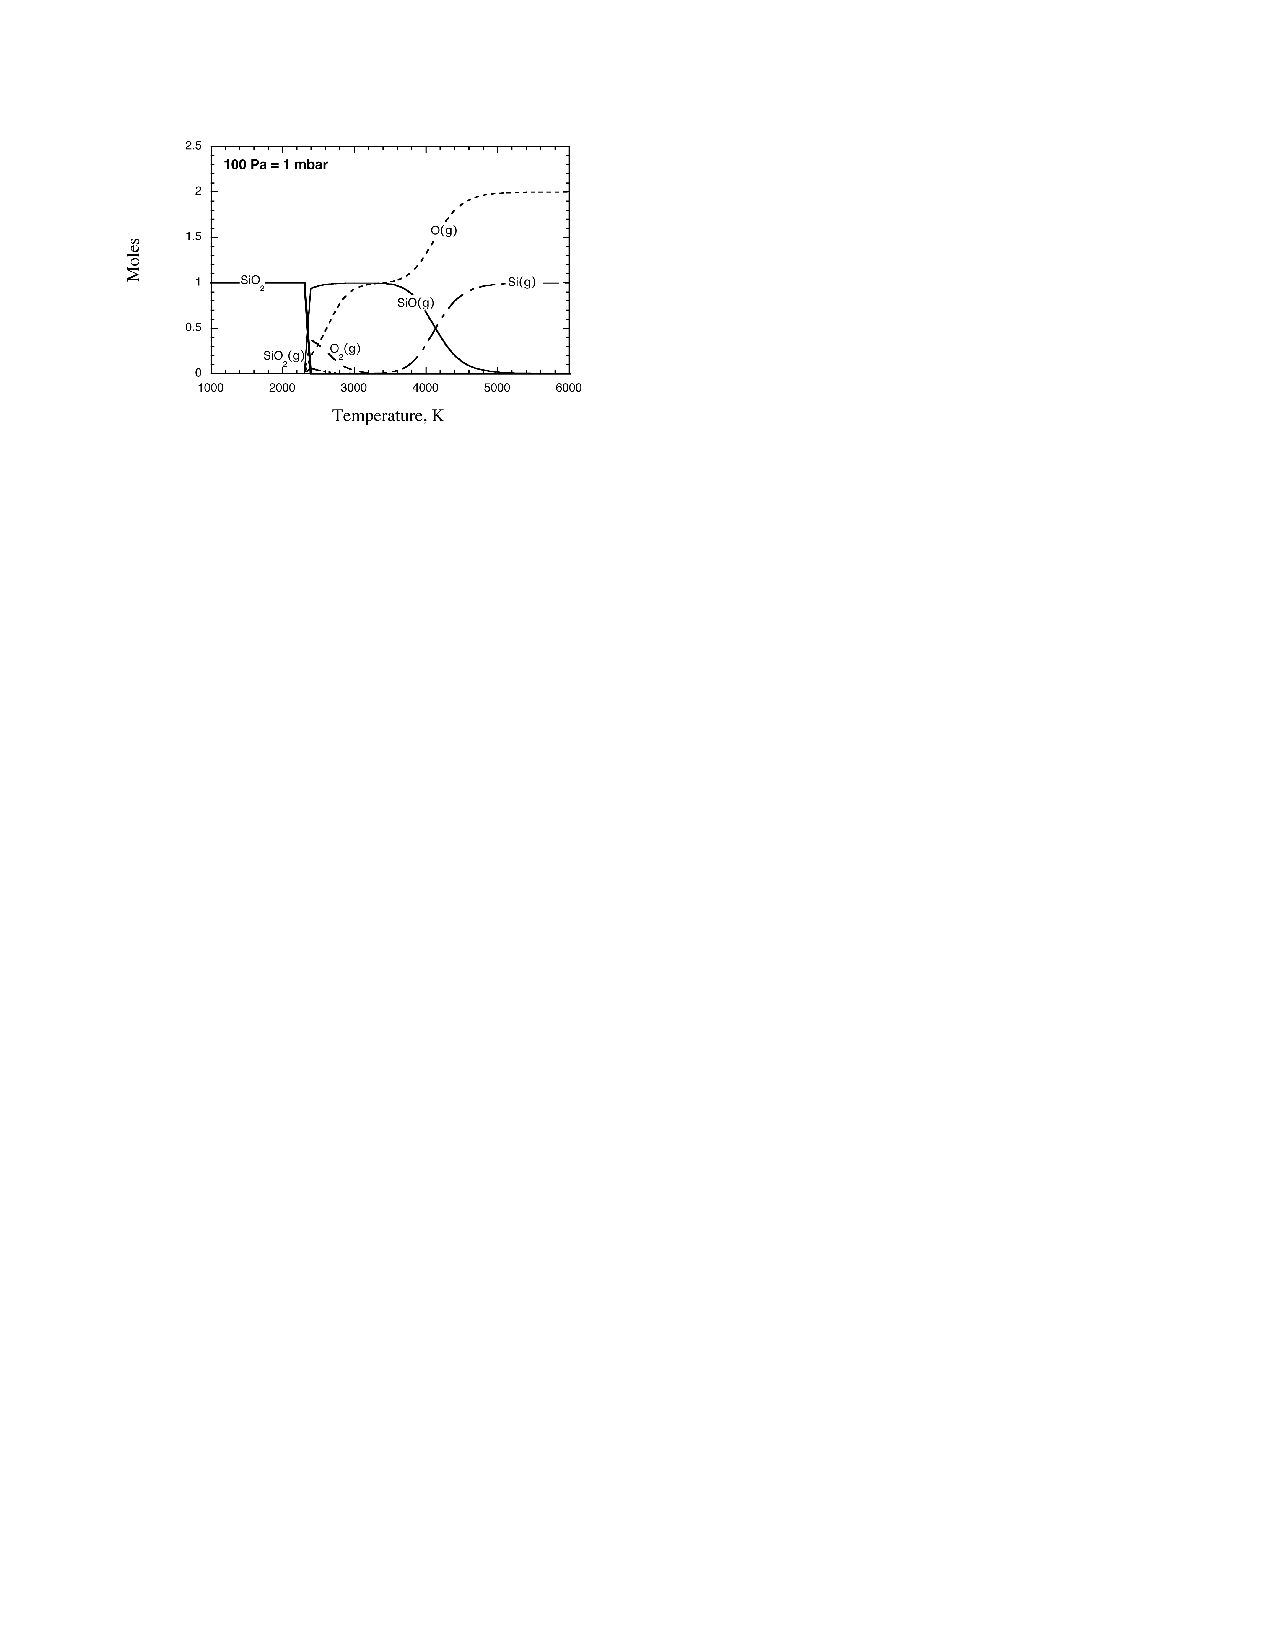
\includegraphics[scale=1.0]{05aneos_phases01}
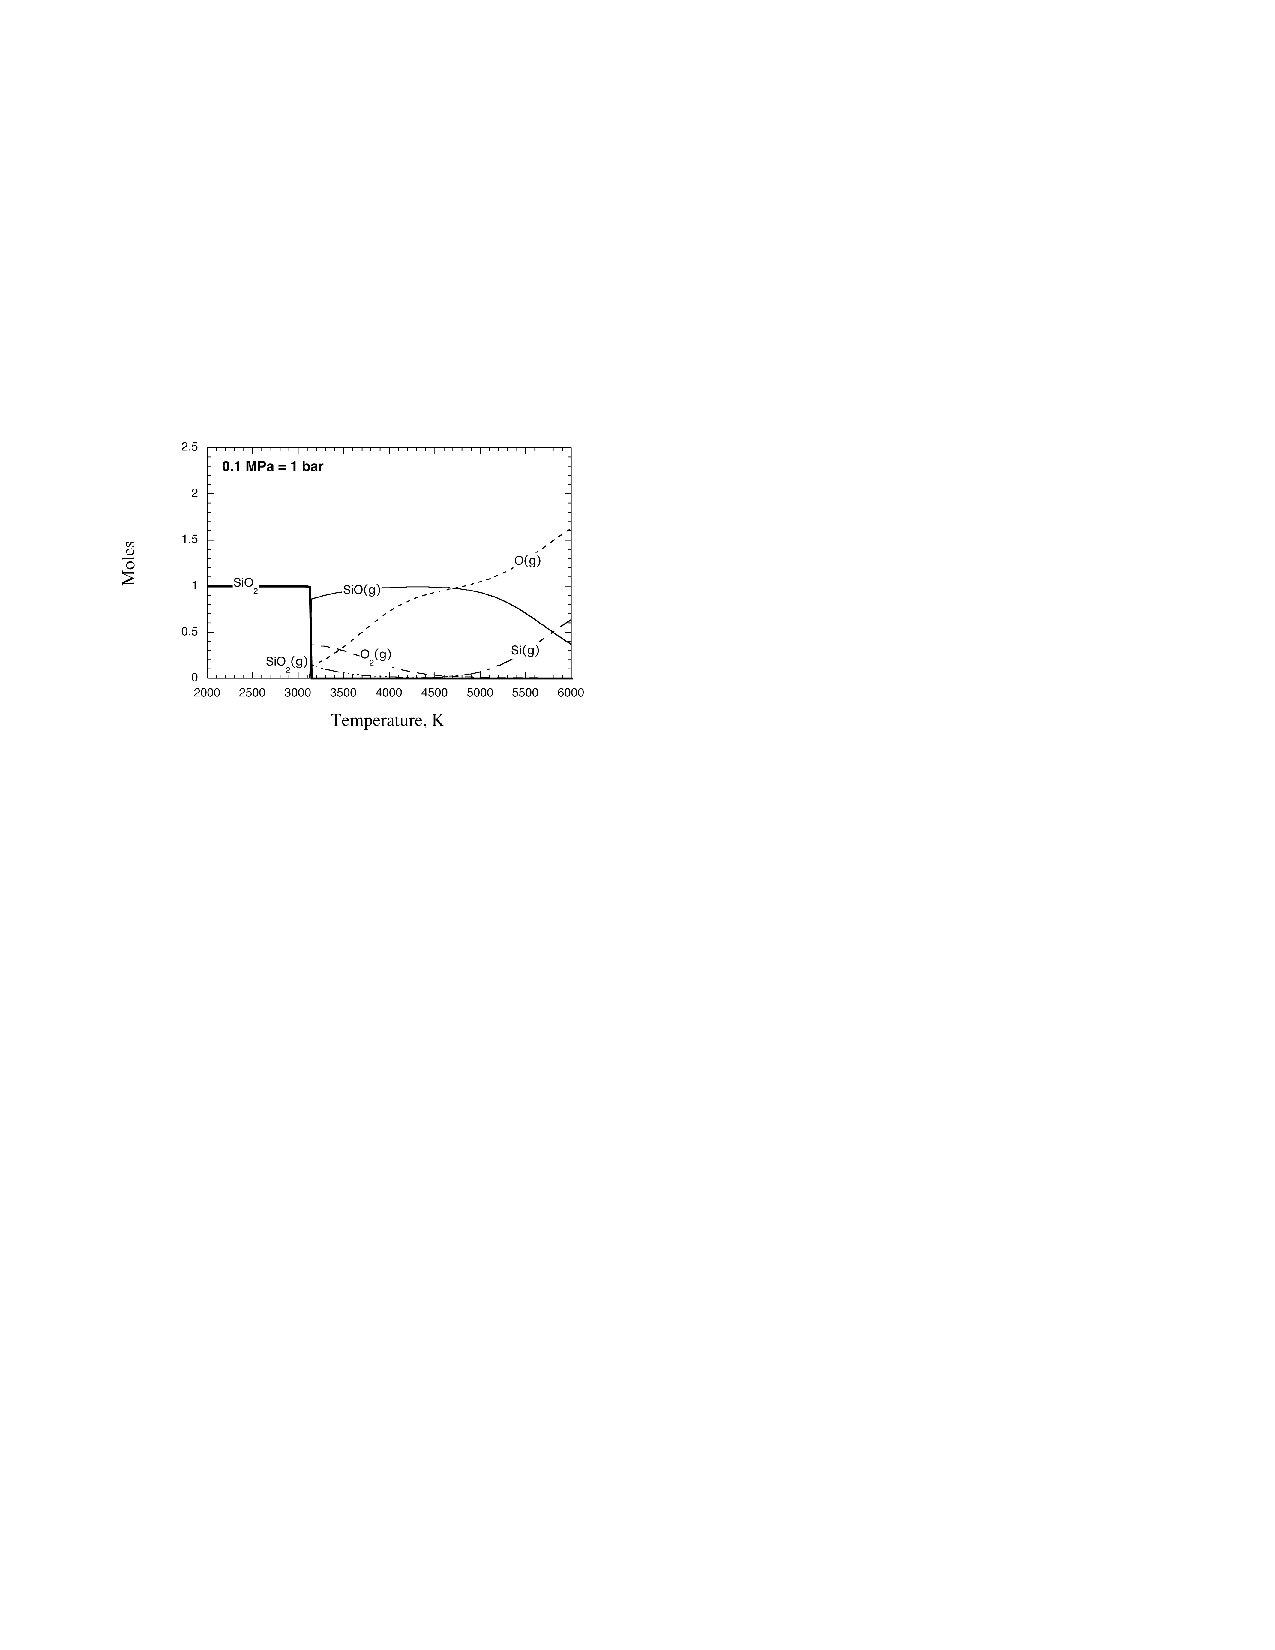
\includegraphics[scale=1.0]{05aneos_phases02}
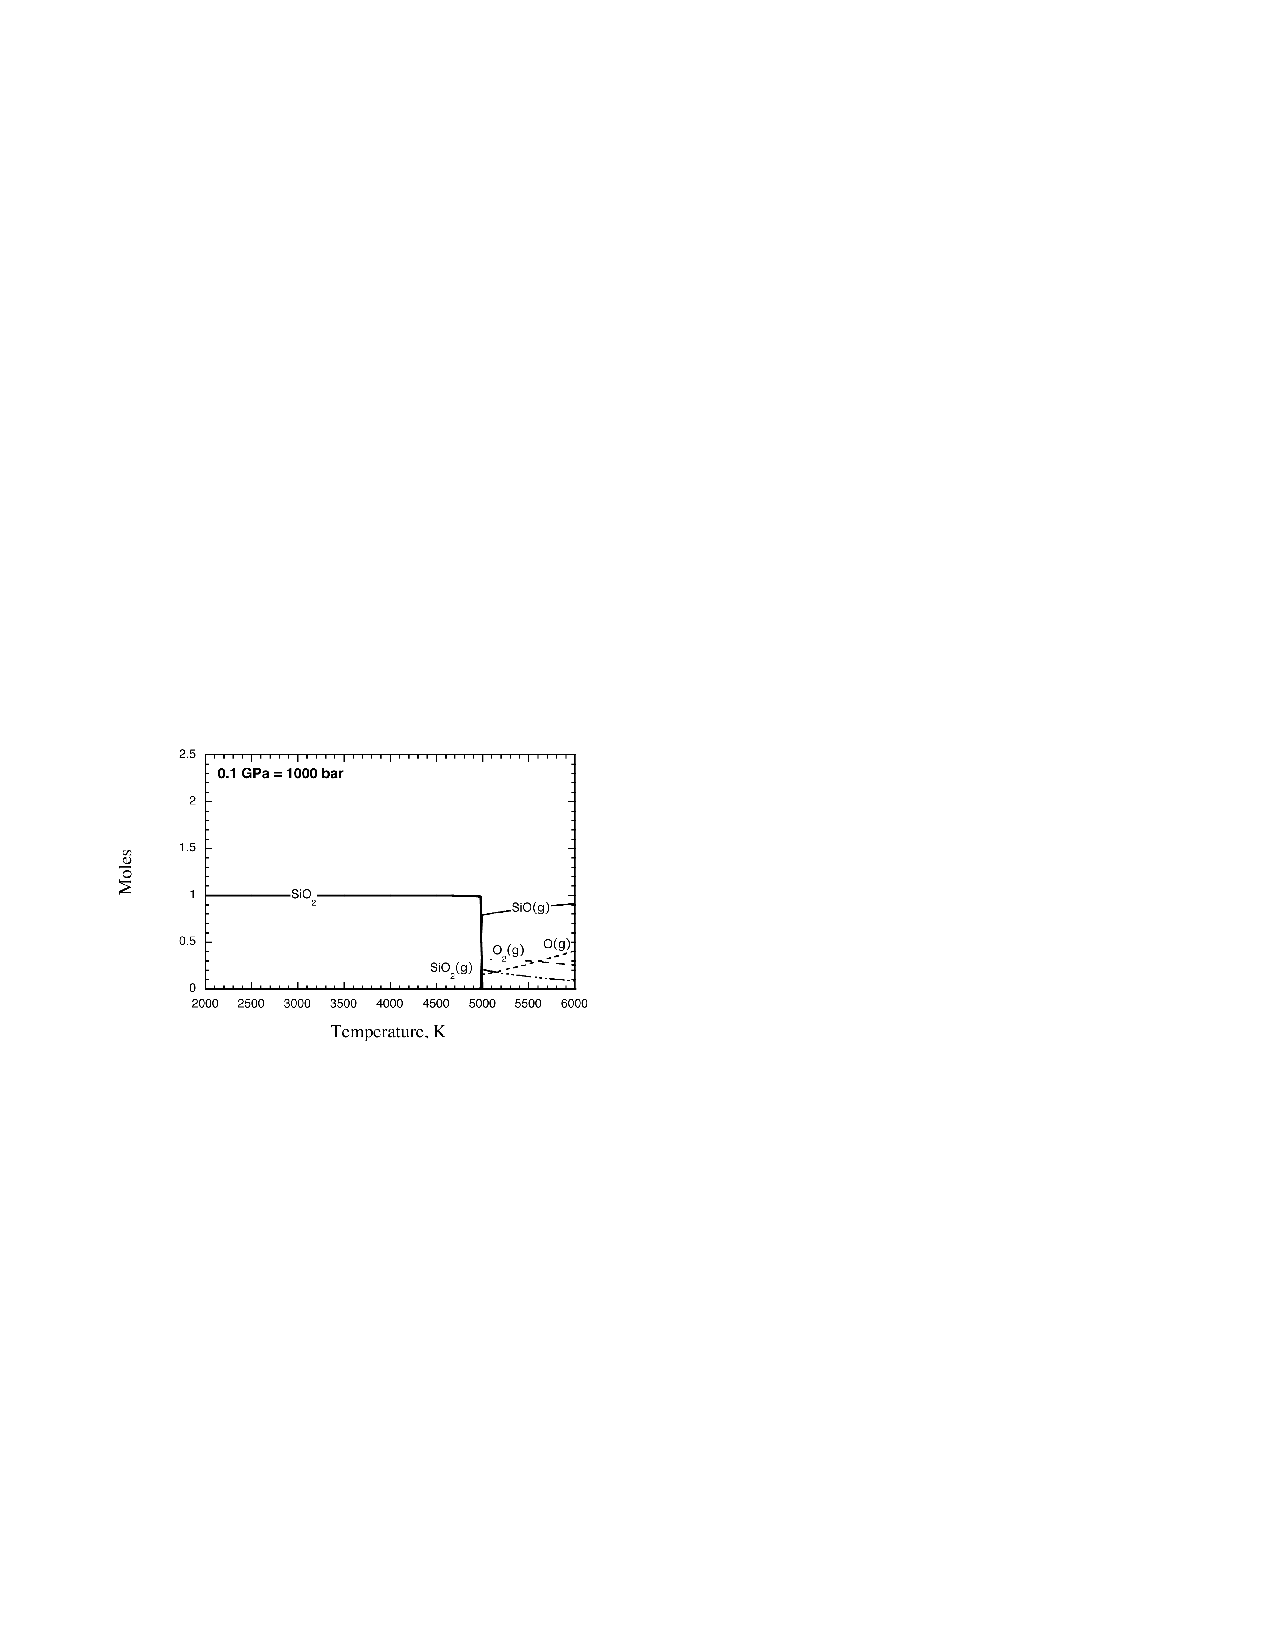
\includegraphics[scale=1.0]{05aneos_phases03}
\caption{Figure 4 from \cite{Melosh:2007p3502} showing the present species depending in pressure and temperature for the $SiO_2$ M-ANEOS equation of state.}
\label{ch02_eos02_fig05}
\end{figure}

ANEOS uses as $(\rho, T)$ as the thermodynamical state variables as input parameters, whereas the hydrodynamical equations for a fluid yield the $(\rho, u)$ or $(\rho, s)$ depending on whether the energy or the entropy equation is solved and integrated. Specific energy and entropy are both returned by ANEOS. Luckily both variables $u(\rho, T)$ and  $s(\rho, T)$ are monotonic increasing functions of temperature, so the correct temperature for given specific energy or entropy can be found through a root finding algorithm. We found the Brent Rooter \cite{Press2002nrc..book.....P} to converge usually within a few iteration steps, for a temperature range covering a few $K$ to a few ten thousand $K$ and a precision of $3 \times 10^{-8}$.

ANEOS dates back to a time, when computer memory was sparse and it was not possible to store large tables of complicated functions. Calling ANEOS itself therefore incorporates numerous internal iteration routines. This iterations over iterations make a single EOS call for given $(\rho, u)$ or $(\rho, s)$ computationally relatively costly. Nowadays memory is abundant. Therefore we tabulate ANEOS, so that EOS calls simply reduce to finding suitable points in the parameter space and interpolating between them. Figures \ref{ch02_eos02_fig02} - \label{ch02_eos02_fig05} show the tables for four different material. The parameter space is given by $(\log \rho, \log u)$ for the density-energy table and $(\log \rho, \log u)$ for the density-entropy table. Each material has a reference density $\rho_0$ at standard conditions. The important shock processes in planetary system collisions between solid or liquid bodies occur at densities roughly inside an order of magnitude above the reference density. At the same time the table needs to cover vaporized material which has a density many magnitudes below the reference values. In order to fulfill both requirements, the table is split into a high- and a low-density region. The high density region spans roughly 2.5 orders of magnitude starting from $100kg/m^3$ with 500 grid points. The low density  region covers the vapor and solid-vapor mixture regions and goes all the way down to $10^{-8}kg/m^3$ with only 100 grid points. This low number of grid points over such a large density range is no problem, because all variables behave sufficiently smooth in this regions and interpolation delivers good agreements to the theoretical values. Specific energy and entropy are tabulated in both tables with 1500 points in the logged value. In the rare case, that a value outside of the table is requested, the code falls back to the iteration routine used to create the tables. 

Figures \ref{ch02_eos02_fig02} - \label{ch02_eos02_fig05} show the phase state information returned by ANEOS. For mixed states, the single density used by ANEOS is the average density for all phases together.

\begin{figure}
\begin{center}
\includegraphics[scale=0.50]{04aneos_phases_mat05}
\caption{Look-up tables for the ANEOS equation of state for iron. The left plot shows the table using density and specific energy as the parameter space, while the right plot shows the table using density and specific entropy. Both tables are divided into two sub-tables. A small table with covers the low-density region and uses 100 equally spaced grid points in logged density from $\rho_{min}$ to $\rho_{med}$ and 1500 points in logged specific energy. In the higher density region from $\rho_{med}$ to $\rho_{max}$, the density resolution is increased by using 500 grid points in logged density, in order the resolve the phase transitions well enough. The same sub-division also applies to the density-entropy table, except that instead of logged specific energy logged specific entropy is tabulated. The colors in the plot indicate the phase information returned by ANEOS. Solid is red. Orange indicates material where partial melting occurs and both a solid and a liquid phase exists. For an increase in energy or entropy, the material liquifies completely, indicated by blue color. Green color indicates the mixed state, where solid, liquid and vapor phases co-exist at the same time. White regions are invalid.}
\label{ch02_eos02_fig02}
\end{center}
\end{figure}

\begin{figure}
\begin{center}
\includegraphics[scale=0.50]{04aneos_phases_mat02}
\caption{The same tables as in \ref{ch02_eos02_fig02} for $H_2 O$ }
\label{ch02_eos02_fig03}
\end{center}
\end{figure}

\begin{figure}
\begin{center}
\includegraphics[scale=0.50]{04aneos_phases_mat04}
\caption{The same tables as in \ref{ch02_eos02_fig02} for \emph{dunite}. In the grey zones, ANEOS returns valid pressures and sound speeds, but does not return any particular phase information.}
\label{ch02_eos02_fig04}
\end{center}
\end{figure}

\begin{figure}
\begin{center}
\includegraphics[scale=0.50]{04aneos_phases_mat01}
\caption{The same tables as in \ref{ch02_eos02_fig04} for the modified M-ANEOS for $SiO_2$}
\label{ch02_eos02_fig05}
\end{center}
\end{figure}


%%
%   G R A V I T Y 
%%
\section{Gravity}
A self-gravitating continuum with the density field $\rho(\rv)$ has the gravitational potential $\Phi(\rv)$ which fulfills the Poisson equation for gravity
\begin{equation}
\label{ch02_sph01_eq038}
\nabla ( \nabla \Phi(\rv) ) = \Delta \Phi(\rv) = 4 \pi G \rho(\rv)
\end{equation}

and acts on the fluid through the external potential term in the Navier-Stokes equation \ref{ch02_fld01_eq002}. Grid codes often find the potential by taking the fourier transform of the Poisson equation, which yields directly the fourier transform of the potential which again can be transformed back again into real space.

When we approximate the density field by discrete particles, self-gravity reduces to the N-body problem, where the potential and gravitational acceleration for particle i is given by
\begin{equation}
\label{ch02_sph01_eq038}
\av_j = - G \sum_{i \ne j} \frac{m_i}{r_{ij}^2} \frac{\rvij}{r_{ij}} 
\end{equation}

Calculating self-gravity with this sum is called direct-summation and involves for a each of N particles a sum with N force terms. So the complexity of this simple algorithm is $O(N^2)$. By making use of the symmetry of the force terms, only half of the force terms need to be evaluated, but the algorithm still retains its $O(N^2)$ complexity. This method is only practical if the problem can be satisfactorily modeled by a small number of particles (a few thousand) and specially designed computers are used (e.g. GRAPE). An example of such an application are the evolution and accretion of a proto-lunar into a Moon as done by \cite{Kokubo:2000p2195}.

\subsection{Multipole approximation}
Different methods exist to avoid the prohibitively high computational complexity of the direct summation method mentioned above.  They all make use of the strong $r^{-2}$ dependence of the gravitational field on distance, which means that the most significant contributions in the direct sum come from the nearest particles for more or less equally massive particles. 


The field of more distant particles can be approximated as background field, which does not have to be resolved down to the contribution of every single particle. Instead, distant particles are summarized into clusters and their field is approximated as the one of a single particle with the cluster's mass $m_C$ at the cluster's center of mass $\rv_C$:

\begin{align}
\label{ch02_grav02_eq001}
\av_j &= - G \sum_{i~\epsilon~C} \frac{m_i}{r_{ij}^2} \frac{\rv_{ij}}{r_{ij}} \approx - G \frac{m_{C}}{r_{Cj}} \frac{\rv_{Cj}}{r_{Cj}} ~~~~ \text{when}~r_{ij} \gg r_{jk} ~~~ \forall j,k ~ \epsilon~C \\
m_C &= \sum_{i~\epsilon~C} m_i ~~~~ \rv_C = \frac{1}{m_C} \sum_{i~\epsilon~C} \rv_i m_i ~~~~ \rv_{Cj} = \rv_j - \rv_C 
\end{align}

This is the \emph{monopole approximation}. In more general terms the total mass of the cluster is the rank-0 monopole tensor $M$ with the center of mass $X$

\begin{align}
\label{ch02_grav02_eq002}
M & = \sum_{c} m_{c} \\
\Xv  & = \frac{1}{M} \sum_{c} m_{c} \rv_{c} ~~~~~~~~ \text{for}~M > 0
\end{align}

We use the same indices as in \cite{McMillan:1993p43}, where $i,j$ number vector components and $c$ indexes particles in a cluster or clusters in a group of clusters. The next highest non-zero multipole term is the traceless rank-2 quadrupole tensor

\begin{equation}
\label{ch02_grav02_eq003}
Q_{ij} = \sum_{c} m_c \big( 3 r_{i, c} r_{j, c} - \rv_{c}^2 \delta_{i j} \big) \\
\end{equation}

where $r_{i,c} = \Xv_i - \rv_{i,c}$ denotes the $i$-th component of the distance vector between a cluster's particle $c$ and the center of mass of the cluster. The rank-3 octupole tensor can be reduced to a rank-2 tensor 

\begin{equation}
\label{ch02_grav02_eq004}
S_{ij}  = \sum_{c} m_c \big[ 5 \big( 3 - 2  \delta_{i j} \big) r_{i, c}^2 - 3 \rv_{c}^2 \big] r_{j, c}\\
\end{equation}

and the single rank-0 component

\begin{equation}
\label{ch02_grav02_eq005}
S_{1 2 3} = 15 \sum_{c} m_c r_{1, c} r_{2, c} r_{3, c}
\end{equation}

Higher order moments are usually not used and skipped here. The field of a group of cluster can be approximated by summing up the multipole moments of the individual clusters $c$. The mass can simply by summed up:

\begin{equation}
\label{ch02_grav02_eq006}
M = \sum_{c} M_{c}
\end{equation}

The quadrupole tensor now also includes the quadrupole moments of the individual cluster:
\begin{equation}
\label{ch02_grav02_eq007}
Q_{ij} = \sum_{c} M_{c} \big( 3 r_{i, c} r_{j, c} - \rv_{c}^{2} \delta_{i j} \big) + Q_{i j, c} 
\end{equation}

and finally the octupole tensor yields:

\begin{align}
\label{ch02_grav02_eq008}
S_{ij} = \sum_{c}&  M_{c} \big[ 5 \big( 3 - 2 \delta_{i,j} \big) r_{i, c}^{2} - 3 \rv_{c}^2 \big] r_{j, c} 
+ 5 \big( 1 - \delta_{i j} \big) r_{i, c} Q_{i j, c} \nonumber \\
&+ \frac{5}{2} r_{j, c} Q_{i i, c} - \sum_{l} \big[ r_{l, c} Q_{j l, c} \big] + S_{i j, c} \\
S_{1 2 3} =& 15 \sum_{c} M_{c} r_{1, c} r_{2, c} r_{3, c} + \frac{5}{3} \big( r_{1, c} Q_{2 3, c} + r_{2, c} Q_{3 1, c} + r_{3, c} Q_{1 2, c} \big) + S_{1 2 3, c }
\end{align}

The center of mass of the group of clusters is simply given by 
\begin{equation}
\label{ch02_grav02_eq009}
\Xv = \frac{1}{M} \sum_{c} M_{c} \Xv_{c} ~~~~~~~~  M > 0
\end{equation}

Note that particles can be treated like clusters with vanishing multipole moments.

The gravitational potential of a cluster can now be approximated by its multipole expansion:
\begin{equation}
\label{ch02_grav02_eq010}
\phi(\rv) = G \bigg(
\underbrace{ - \frac{M}{r} }_{monopole} ~ 
\underbrace{ - \frac{Q_{i j}}{r^{3}} \frac{r_{i} r_{j} }{2 r^{2} } }_{quadrupole}~ 
\underbrace{ - \frac{S_{i j}}{r^{4}} \frac{r_{i}^2 r_{j}}{2 r^{3} } + \frac{ S_{1 2 3} }{r^{4}}\frac{ r_{1} r_{2} r_{3} }{2 r^{3}} }_{octupole}~ 
+ O\Big(\frac{1}{r^{7}}\Big) \bigg)
\end{equation}

and so the acceleration for a point mass at $\rv$ in this potential yields

\begin{align}
\label{ch02_grav02_eq011}
a_{k} &= - \nabla_{k} \phi(\rv) \approx - G \bigg(
\underbrace{ \frac{M}{r^{2}} \frac{r_{k}}{r} }_{monopole}+ 
\underbrace{ \frac{Q_{i j}}{r^{4}}
\big( \frac{\delta_{i k} r_{j} }{r} + \frac{5 r_{i} r_{j} r_{k} }{2r^{3}} \big)
}_{quadrupole} \nonumber \\
&+ \underbrace{ \frac{S_{i j}}{r^{5}}
\big( \frac{ \delta_{i k} r_{i} r_{j} }{r^{2}}
+ \frac{ \delta_{j k} r_{i}^{2} }{2 r^{2} }
- \frac{7 r_{i}^{2} r_{j} r_{k} }{r^{4} } \big) 
 + \frac{S_{1 2 3}}{r^{5} }
\big( \frac{\delta_{1 k} r_{2} r_{3} + \delta_{2 k} r_{3} r_{1} + \delta_{3 k} r_{1} r_{2}}{2 r^{2}} 
- \frac{7 r_{1} r_{2} r_{3} r_{k} }{2 r^{4}}\big) 
}_{octupole}
\bigg)
\end{align}

\subsection{Barnes and Hut Tree}
\cite{Barnes:1986p2853} describe an algorithm, where particles are grouped into cluster with the help of a Tree. But first we need to know a few basic things about trees: A graph is a set of elements represented by \emph{nodes}. A tree is a rooted, directed graph in which any two nodes are connected by one and only one path. One node is defined as the \emph{root node}.

Each node can have a number of children\footnote{often the term \emph{daughter} is used, but because of the asexual nature of tree nodes we are using here the term \emph{child}} 
nodes and has exactly one parent, expect for the root node which has no parent. Nodes can be assigned a depth. The root node per definition has depth $0$ and the children of a node have the inherit the depth of the parent increased by one. Figure \ref{fig:simpletree} shows a simple tree. The blue square represents the root node and has two children with depth 1, while on of this children has again two children with depth 2. Tree data structures are usually drawn upside-down, this means with the root on top and increasing depth to the bottom.

\begin{figure}[htbp]
\begin{center}
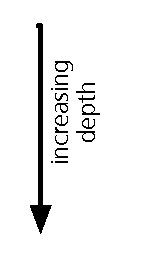
\includegraphics[scale=1.0]{10tree_depth.pdf}
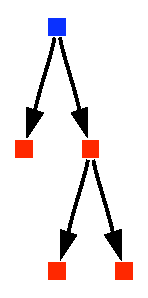
\includegraphics{08simpletree.pdf}
\caption{A simple tree. Squares represent nodes which are interconnected by arrows pointing from the parent node to its children. The blue square is called the root node and has depth $0$.}
\label{ch02_grav02_fig01}
\end{center}
\end{figure}

Nodes without children are called \emph{leaf nodes}. A disjoint set of trees is called a \emph{forest}. One notices that the definition for a tree does not only fit the whole set of nodes of a tree, but also subsets. Every node can be taken as a root node and forms again a tree, also called a \emph{subtree} of the tree. Or one can say, that the children of a node form a forest of trees.

A tree datastructure can be used to recursively subdivide space. The basic idea is to take a volume, assign this volume to a node in a tree, then subdivide this volume in disjoint subvolumes and assign them to the children of the node. The subdivision of space can be mapped onto a tree. The easiest form of subdivision is using volumes which are aligned with the spatial dimension and have the same sidelength in each dimension. In 2D this corresponds to squares and in 3D to cubes along the axis. This volumes are then divided along each dimension into two equal-length intervals, which leads to $2^d$ subvolumes in $d$ dimensions. So if we have an arbitrary volume with a minimum $x_{i,min}$ and a maximum $x_{i,max}$ in each coordinate $i$ we can enclose this volume with a volume with sidelength $l$ and the center $x_{i,c}$

\begin{equation}
\label{ch02_grav02_eq012}
l = \max_{i} ( x_{i,max} - x_{i,min})  ~~~~ x_{i,center}= \frac{ x_{i,min} + x_{i,max} }{2}
\end{equation}

The $2^{d}$ subvolumes indexed with $j$ have a side length of $\frac{l}{2}$ and center vector components $i = 0 \dots d$, where $d_{i}$ stands for $i^{th}$ digit of the binary representation of the subvolume index $j$

\begin{equation}
\label{ch02_grav02_eq013}
x_{i, j~center} = x_{i,center} + l \frac{(-1)^{d_{i} + 1}}{2} ~~~~~ d_{i} = \frac{j  - \sum_{k \ne i} ( j \mod 2^{k} )}{2^{i}}
\end{equation}

In 2D this subvolumes are called \emph{quadrants}, in 3D \emph{octants}. The corresponding trees to which this subdivision can be mapped to are called \emph{quadtrees} and \emph{octrees}, having up to 4 and 8 children per node.

The Barnes \& Hut algorithm described in \cite{1986Natur.324..446B} subdivides the computational universe containing $N$ gravitationally interacting particles in subvolumes, called \emph{cells}. The particles are children of cell nodes. The tree must be built in a way, that a subvolume of a cell, an octant in 3D, contains no more than one particle. If it does, the subvolume can be again subdivided into a number of cells until the requirement is fulfilled. An example of such a tree is shown in figure \ref{fig:2D_BHtree} for 50 randomly distrbuted particles in 2D. We note that no cell contains more than one particle. Shown below is the corresponding quad-tree to this subdivision of space for the particles

\begin{figure}[htbp]
\begin{center}
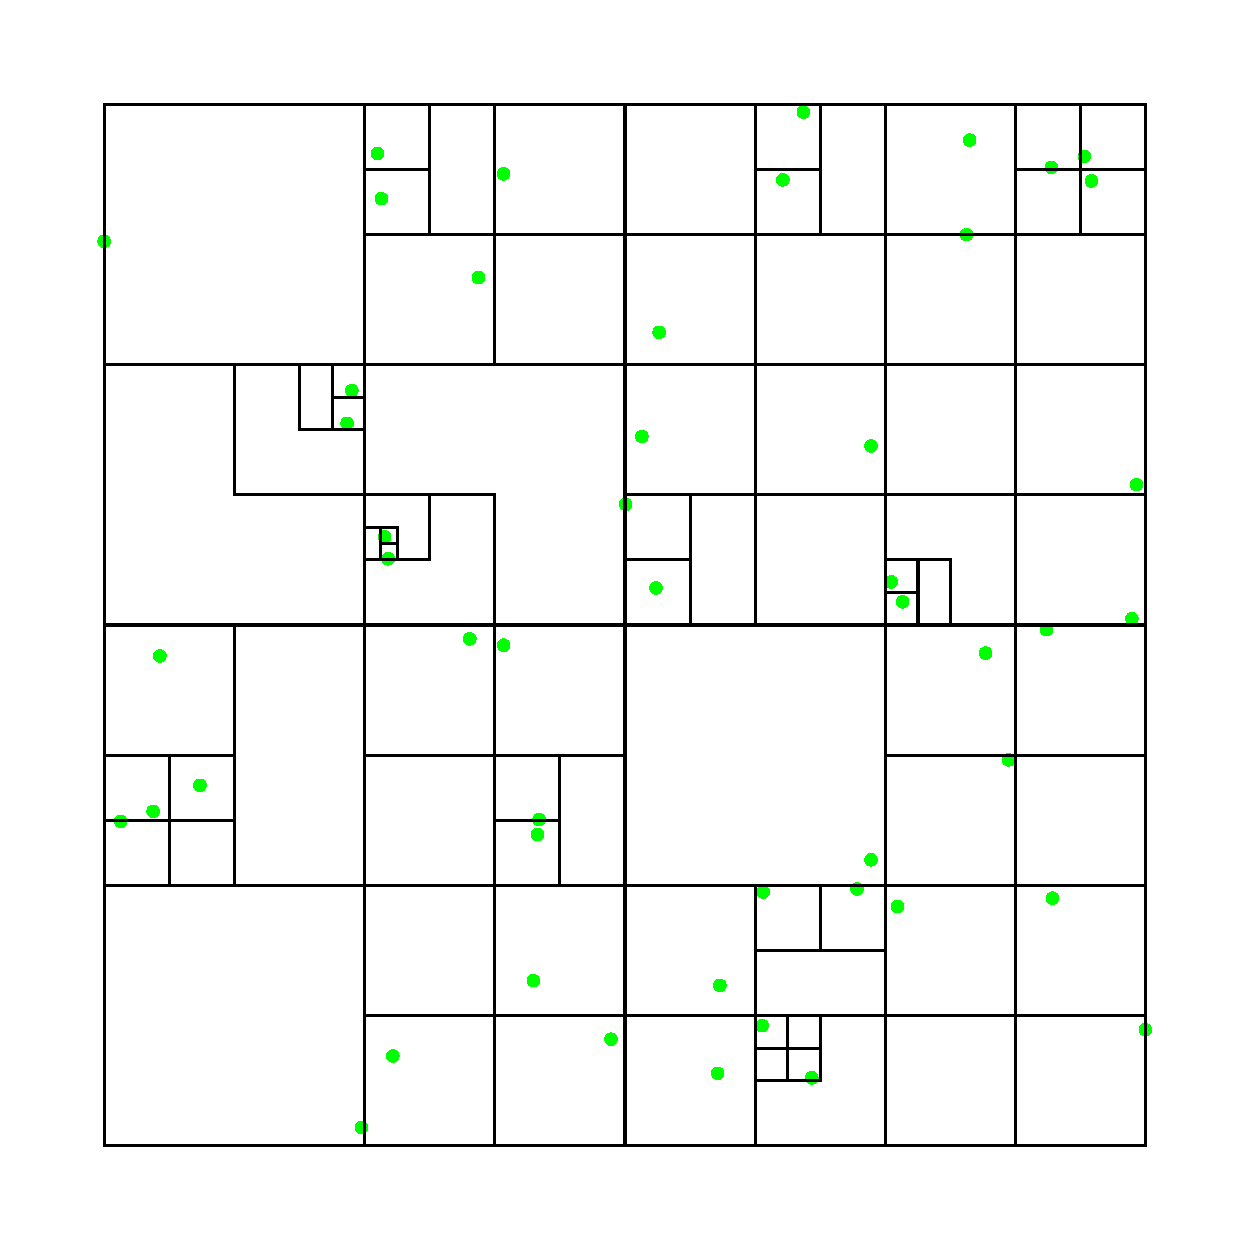
\includegraphics[scale=0.6]{06quadtree50_xy.pdf}
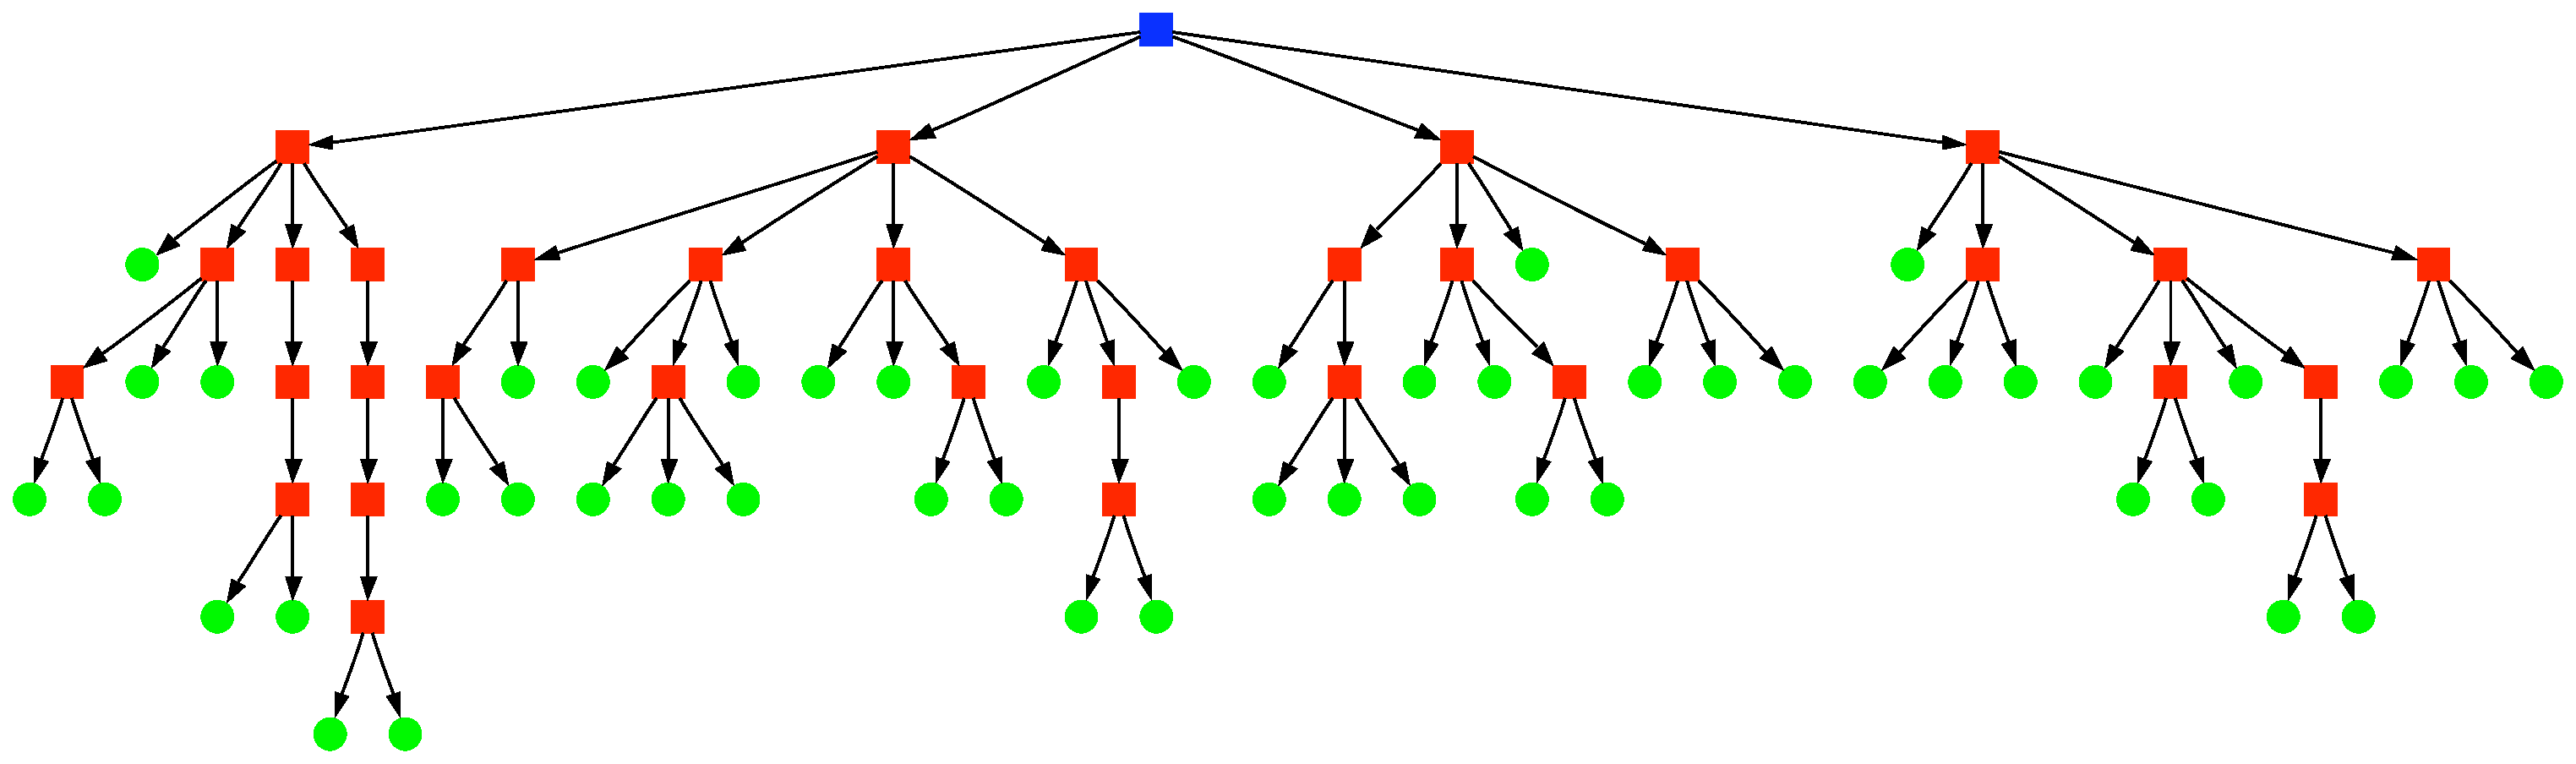
\includegraphics[scale=0.3]{06quadtree50.pdf}
\caption{50 particles randomly distributed in $2D$ and the subdivision into cells (upper plot). The corresponding quad-tree is shown in the figure below. Green dots the represent the particles, while red squares indicate cell nodes. The root cell node is highlighted as a blue square.}
\label{ch02_grav02_fig02}
\end{center}
\end{figure}

Each cell in the tree represents now a clump of particles. For each cell a center of mass and its multipole moments can be calculated. This calculation is done \emph{bottom-up}, so that the multipole moments of the children of node are already calculated, when the multipole moments of the node itself are to be calculated. This can order can be assured with a pre-order tree walk, which will be discussed later. We end up finally with a tree of multipole moments for all the particle clumps given by the subtrees in the tree.

For each particle the acceleration due to gravity can now be calculated according to equation \ref{ch02_grav02_eq011}. The multipole approximation only holds, when then size of the particle cluster is small compared to distance of the particle to the center of mass of the cluster $r_{part- cell}$. A good measure for the size of cluster is the cell size $l$, in which it is contained. The cluster cannot be bigger than the cell and it is usually not smaller by magnitudes expect in pathological cases. The cell sizes get smaller by descending in the tree, so that depending of the particle-cell distance the cell size gets small enough to use the multipole approximation. To decide whether it is necessary to descend further down in the tree, the \emph{multipole acceptance criteron} short \emph{MAC} is used. The one proposed by \cite{1986Natur.324..446B} is

\begin{equation}
\label{ch02_grav02_eq013}
\frac{l}{r_{part-cell}} \le \theta ~~~~ \theta = 0.6 \dots 1.0 ~~~~ r_{part-cell} = | \Xv - \rv_{part}|
\end{equation}

where $\theta$ is the \emph{opening angle} chosen depending on the desired accuracy. The smaller the opening angle, the more accurate the calculation becomes. When $\theta = 0$ no particle cluster cell fulfills the MAC and the tree walk is completed down to each particle, leading again to the direct summation with complexity O($N^2$). For $\theta \ge 1$ an additional error may be introduced, as depending on the distance form the particle to the center of mass of its own cluster the MAC may be fulfilled, leading to a acceleration calculation based on the multipole moments which include the particle itself. This error is called \emph{self-acceleration}. The choice of the MAC determines directly the efficiency and prescision of the Barnes \& Hut method.

\begin{figure}[htbp]
\begin{center}
\includegraphics[scale=0.8]{09bfcomp}
\caption{The left plot shows the relative acceleration errors, due to the multipole approximation $\Delta_{\av_{mp}} = \frac{|\av_{mp}| - |\av|}{|\av|}$ for a self-gravitating spheres using an opening angle $\theta = 0.7$. For all three resolutions, the relative errors are below $10^{-3}$ for more than 90\% of the particles. 
The right plot shows the execution time for one self-gravity run for the Barnes \& Hut tree and the brute force direct summation for different numbers of particles and an opeing angle of $\theta = 0.7$. The code used is the SPHLATCH v2 implementation discussed below with one CPU. Direct summation execution time follows a $O(N^2)$ scaling (dashed line), while the Barnes \& Hut tree shows a more complex scaling. Speed-ups ($\times 20-190$) are considerably for moderate number of particles.}
\label{ch02_grav02_fig03}
\end{center}
\end{figure}


%%
%   I M P L E M E N T A T I O N
%%
\subsection{Tree implementation and algorithms}
The actual implementation of the Barnes \& Hut method described above consists of two main parts: The tree data structure and the algorithms which are applied onto the data structure.

All the information of the tree lies in the nodes: They contain information about their connection to the parent node and to possible children. Additionally they also contain a payload, the information about the volume in space they represent, like the center, the center of mass and the multipole moments of the particles contained in the cell. 

In modern programming languages like FORTRAN or C, the most common approach for implementing a tree data structure, is to define node data structures and then dynamically allocate them in memory. Connections between the nodes can be realized with pointers, pointing to other nodes in the tree. Walks in the tree can then be performed by following those pointer from node to node. Figure \ref{ch02_grav02_fig04} shows the content of a cell node and two particle nodes in an octree. Not shown is the payload data. Both types of node have a pointer to the parent node, so that also upward walks in the tree are possible. The cell node additionally has eight pointers to possible children. If there is no child for the corresponding sub-volume, the pointer has a special value so that it becomes clear that the pointer is invalid. The \emph{next} and \emph{skip} pointers will be explained later.

Tree walks can now be performed in such a tree data structure by defining a current pointer, which points to the current node being processed in a tree walk. By setting this pointer to a child or a parent of a node, movements in the tree can be performed. 

\begin{figure}[htbp]
\begin{center}
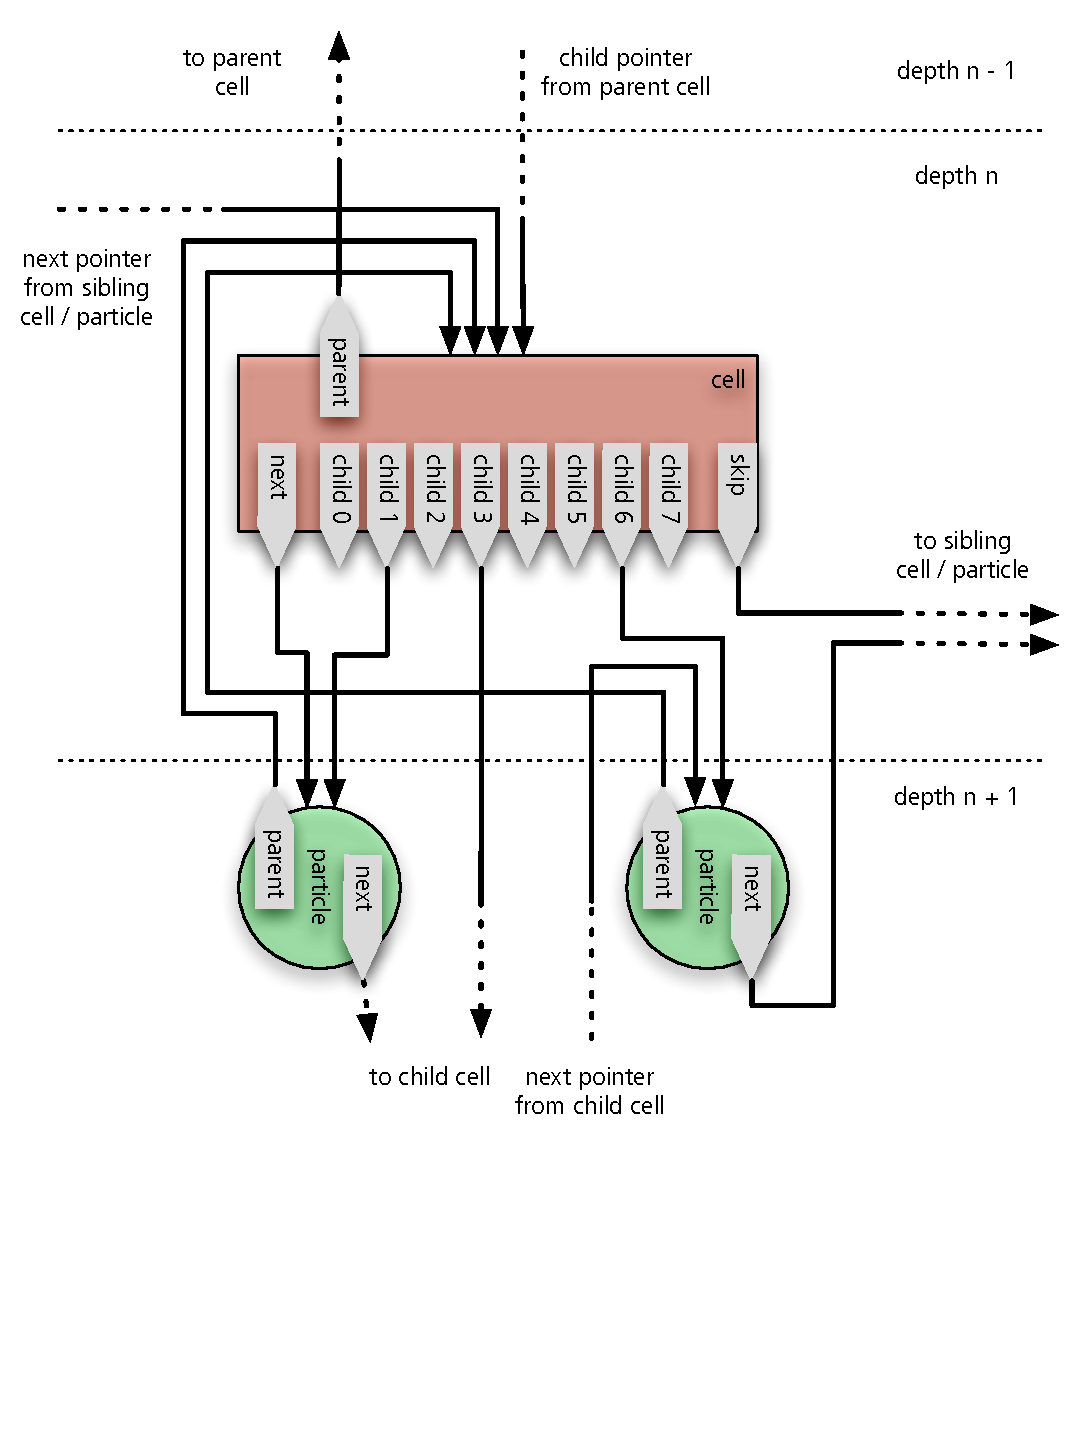
\includegraphics[scale=0.6]{11cell_wiring.pdf}
\caption{Wiring scheme of an octree cell node a depth $n$ with particle childs in subvolume 1 and 6 and a cell node as child 3. Parent pointers allow going upwards in the tree, child pointers downwards. Following the next pointers results in a pre-order tree traversal, where taking the \it{skip} pointer skips a cells subtree.}
\label{ch02_grav02_fig04}
\end{center}
\end{figure}

With the root node as the starting point, there exist two particular ways of traversing the tree downward and applying an action to every encountered node : Pre-order and post-order traversal. Both traversals can be realized with recursive algorithms. Figure \ref{ch02_grav02_fig05} shows the two algorithms: The post-order algorithm first executes itself on the children and performs the action after that. So the action is always performed on a child, before it is performed on its parent. This algorithm is therefore suited for calculations like the multipole summation, where the multipole moments of a cell depend on its children. The pre-order algorithm works exactly the other way round: First the action is performed on the parent node and only after that the algorithm executes itself recursively on the children.

\begin{figure}[htbp]
\begin{center}
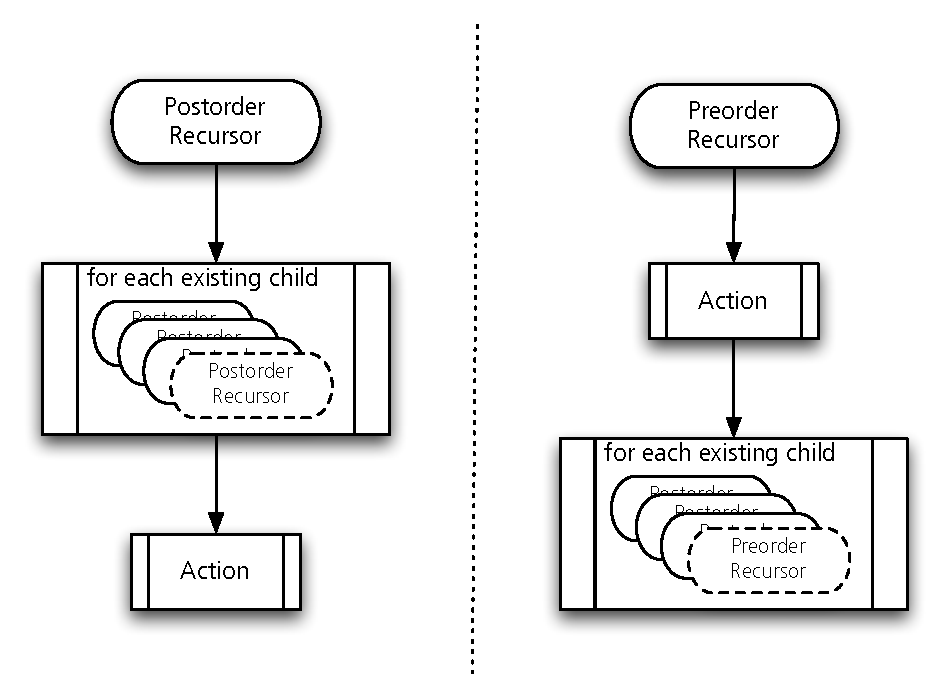
\includegraphics[scale=0.6]{12orderwalks.pdf}
\caption{Post-order vs. pre-order recursors}
\label{ch02_grav02_fig05}
\end{center}
\end{figure}

The Barnes \& Hut tree gravity calculation method requires the following tree algorithms: Inserting particles into the tree, calculating multipole moments, approximating the self-gravity forces and finally the tree also needs to be deleted again. All those algorithms can be derived from two walks presented above.

Figure \ref{ch02_grav02_fig06} shows the tree insertion algorithm. For a particle which was not yet  inserted into the tree, the walk starts at the root node. The sub-volume where the particle is included is checked for an existing node. If there is no node, a new particle node is created there and the algorithm terminates. If there already exists a cell node, the algorithm simply opens the cell and executes ifself at the current position. The third possibility is, that there already exists a particle node (B). In that case particle B is replaced by a cell node and the particle is placed as a child of the new cell. The particle inserter is then run again at the position of the new cell. This algorithm has complexity $N \log{N}$ for $N$ particles, as it has to be executed $N$ times and the depth of the tree goes on average with the factor of $\log{N}$
\begin{figure}[htbp]
\begin{center}
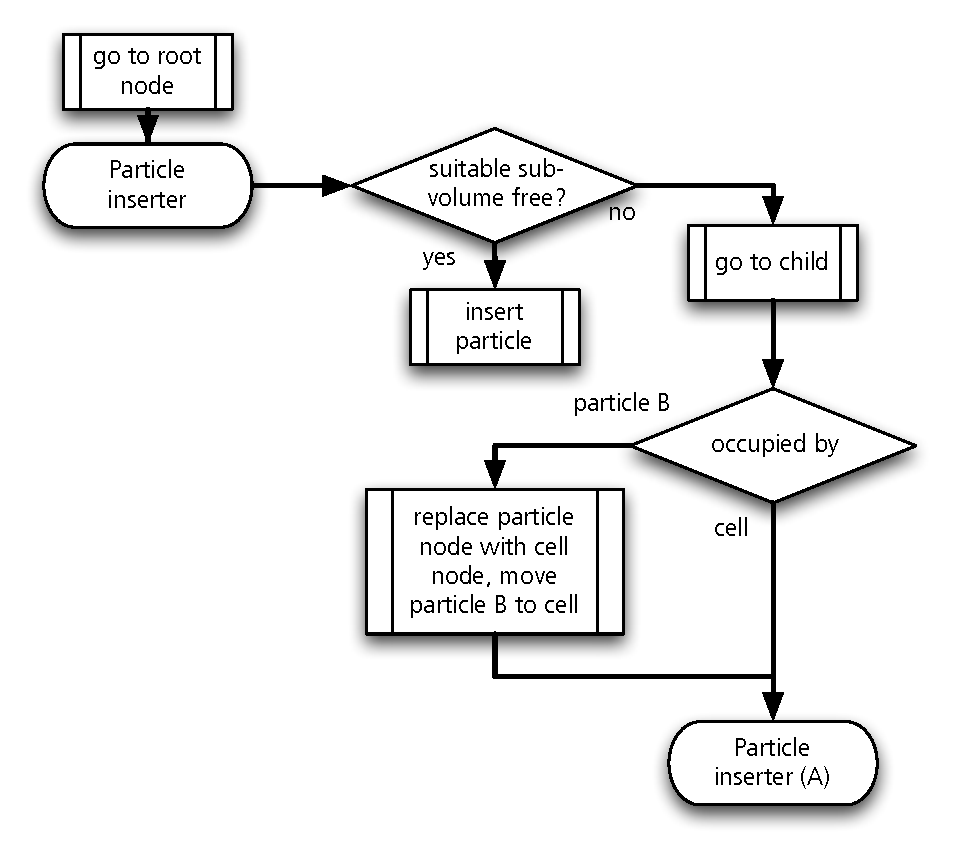
\includegraphics[scale=0.6]{13algo_particle_insert.pdf}
\caption{Algorithm for the insertion of particle A.}
\label{ch02_grav02_fig06}
\end{center}
\end{figure}

As mentioned before, the multipole moments can simply be calculated by a recursive post-order algorithm. Figure \ref{ch02_grav02_fig07} shows the corresponding algorithm. Tree deletion can also be accomplished by using a post-order recursive algorithm, which can be seen on the right side of figure \ref{ch02_grav02_fig07}. Deleting the children of a cell before the cell itself guarantees, that all cells are still connected to the tree until they are deleted.


\begin{figure}[htbp]
\begin{center}
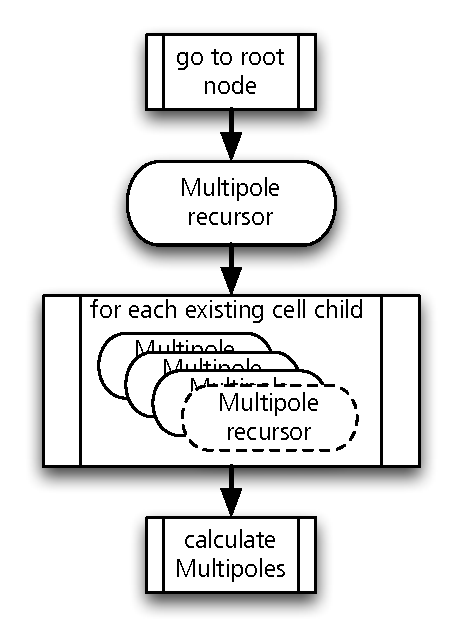
\includegraphics[scale=0.6]{14algo_multipoles.pdf}
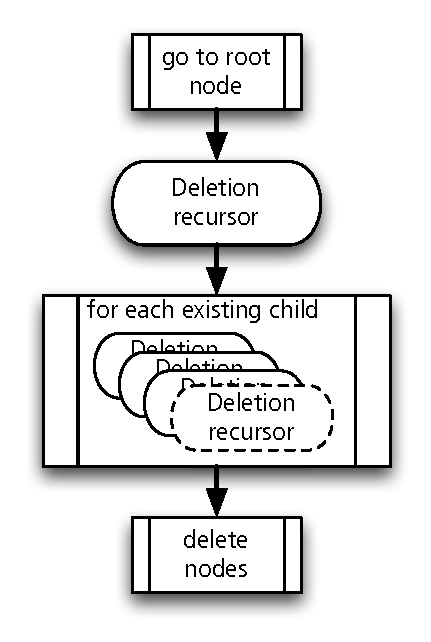
\includegraphics[scale=0.6]{15algo_treedelete.pdf}
\caption{recursive algorithms for calculating the multipole moments in the tree and for deleting all tree nodes. Note that the recursive part of the algorithm does not include going to the root node.}
\label{ch02_grav02_fig07}
\end{center}
\end{figure}

Recursive algorithms are implemented in a procedural language like C or FORTRAN, as functions calling themselves recursively. While implementing tree algorithms in a recursive way results in simple algorithms, it introduces a performance penalty. Calling a procedure introduces a computational overhead \citep{bryant2010computer}. It is therefore desirable to implement the most costly tree algorithms in a non-recursive way. This can be done with the introduction of \emph{next}- and \emph{skip} pointers. The basic idea is to store the next node a certain tree walk would end up at for each node. Figure \ref{ch02_grav02_fig08} shows an example of a small tree. The grey arrows depict the connections between the tree nodes. The black arrows in the middle part of the figure now show the \emph{next}-pointers, which point to the next node in a tree walk compromising all tree nodes. Note that all tree nodes have a \emph{next}-pointer. Another useful pointer for the Barnes \& Hut algorithm is the \emph{skip}-pointer. It points to the next node the tree walk leads too, if the cell node is accepted by the multipole acceptance criterion and its subtree is therefore skipped. The right part of figure \ref{ch02_grav02_fig08} shows the skip pointers for the small example tree. A \emph{skip}-pointer of a cell always points to a sibling node at the same or a smaller depth than the cell. It is crucial, that it only skips the subtree of its own cell and no other cells. 

\begin{figure}
\begin{center}
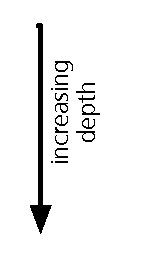
\includegraphics[scale=0.80]{10tree_depth.pdf}
\includegraphics[scale=0.35]{10tree_no_ptr.pdf}
\includegraphics[scale=0.35]{10tree_next_ptr.pdf}
\includegraphics[scale=0.35]{10tree_skip_ptr.pdf}
\caption{An excerpt from a  tree with particles at different depths. Grey arrows depict the connections between the tree nodes. In the middle plot, the \emph{next}-pointers are shown. Following them results in a post-order tree walk along all nodes. The very last \emph{next}-pointer The right plot shows the \emph{next}-pointers, lead to the next node with an equal or smaller depth. This \emph{next}- and \emph{skip} pointers allow tree walks to be implemented with non-recursive algorithms.}
\label{ch02_grav02_fig08}
\end{center}
\end{figure}

The two most costly tree algorithms, the gravity walk and the neighbor search, can now be realized in a non-recursive way. Figure \ref{ch02_grav02_fig09} shows the flow diagram for the gravity walk for evaluating the gravity acceleration on particle A. The current pointer is set to the root node and the walk starts. First it is checked, whether the current pointer still points to a valid node. If not the walk has terminated. If the node is valid, the type of the node is checked. If the node is a cell node, the multipole acceptance criterion is evaluated. In case the MAC is fulfilled, the multipole moments of the cell are used to approximate the gravity force all particles represented by this cell node onto the single particle the force has to be evaluated for. After that, following the \emph{skip} pointer leads to the next node in the tree. In case the evaluated node is a particle, its interaction with particle A is calculated, when the particle node does not correspond to the one representing particle A itself. This algorithm has the complexity $\log{N}$ for one particle and $N \log{N}$, although \cite{1986Natur.324..446B} note that the scaling in reality is more like $N$.

\begin{figure}[htbp]
\begin{center}
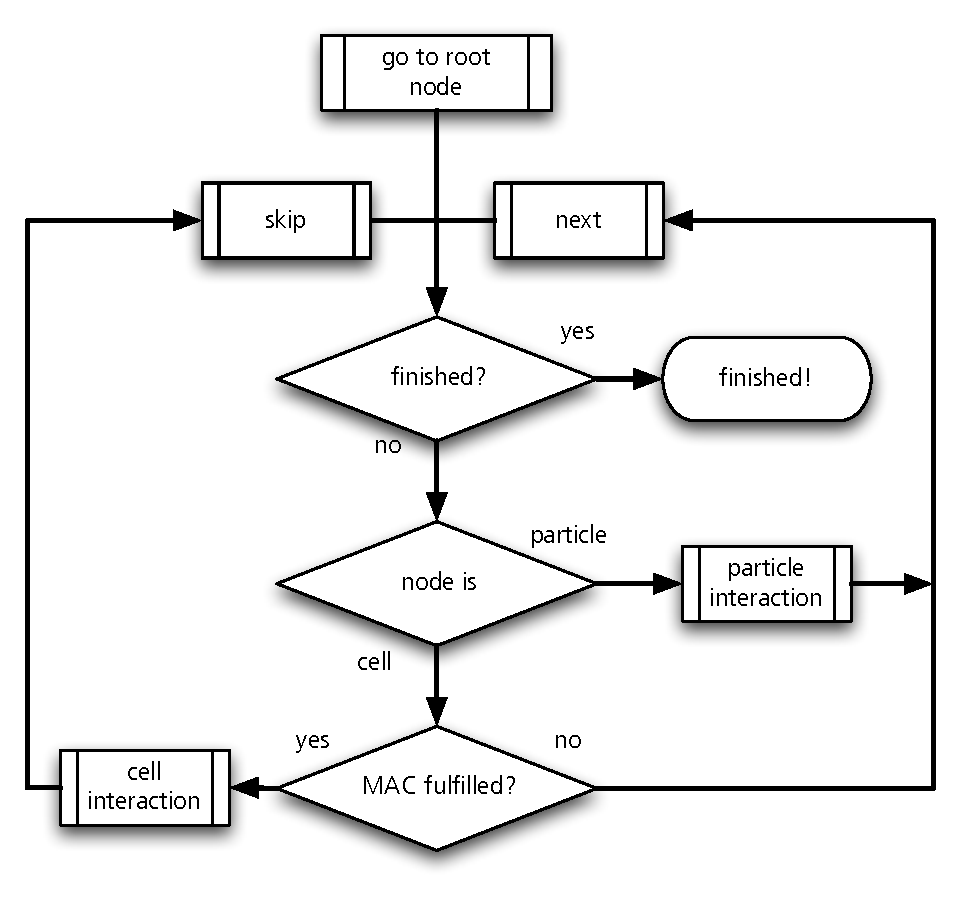
\includegraphics[scale=0.6]{19algo_gravwalk.pdf}
\caption{A non-recursive algorithm for the Barnes \& Hut tree walk.}
\label{ch02_grav02_fig09}
\end{center}
\end{figure}

Searching for particle A's neighbors can be done as shown in figure \ref{ch02_grav02_fig10}. The basic idea of the algorithm is to first find the cell which fully encloses the search sphere around the particle for which the neighbors should be found. This cell is then the root of the subtree where all the potential neighbors can be found. The algorithm starts by setting the current pointer to the particle node of the particle for which the neighbor search is done. The tree is traversed upwards until a cell is reached, which fully enclosed the search sphere given by the particles position and the search radius around it. If this criterion is fulfilled can be simply checked by comparing the edges of the cell to the most extreme coordinate of the search sphere in each dimension. From here on the subtree is searched for neighbors. If a particle node is encountered, its distance to the original particle A is checked and if it's inside the search radius, the neighbor function is executed for this particle node. In case the neighbor search is used for SPH, this function is simply a sum term executed on the neighbor. Alternatively if an actual list of neighbors is required, the function simply adds the neighbor particle to this list. If the node in the subtree search is a cell node, it is checked, whether the cell is completely outside the search sphere. If so, the cell is skipped, if not it is opened by following the \emph{next}-pointer. The algorithm is finished, if the search subtree has been traversed. This is the case, if the current pointer points to the \emph{skip}-pointer of the search subtree root node, the one which fully enclosed the search sphere. A nice property of this search algorithm is, that it's complexity is constant. The size of the search subtree does only depend on the size of the search sphere and not on the size of the total tree. Neglecting performance penalties due to caching issues, the algorithm has the same performance independent of the total number of particles. Note that this scaling is only possible, because of the very first step in the algorithm, where the current pointer is set directly to the particle node. This is achieved by storing a pointer to the particle node at the time of particle insertion into the tree. The penalty of storing an extra pointer into the tree for each particle is small, compared to the gain in speed.

\begin{figure}[htbp]
\begin{center}
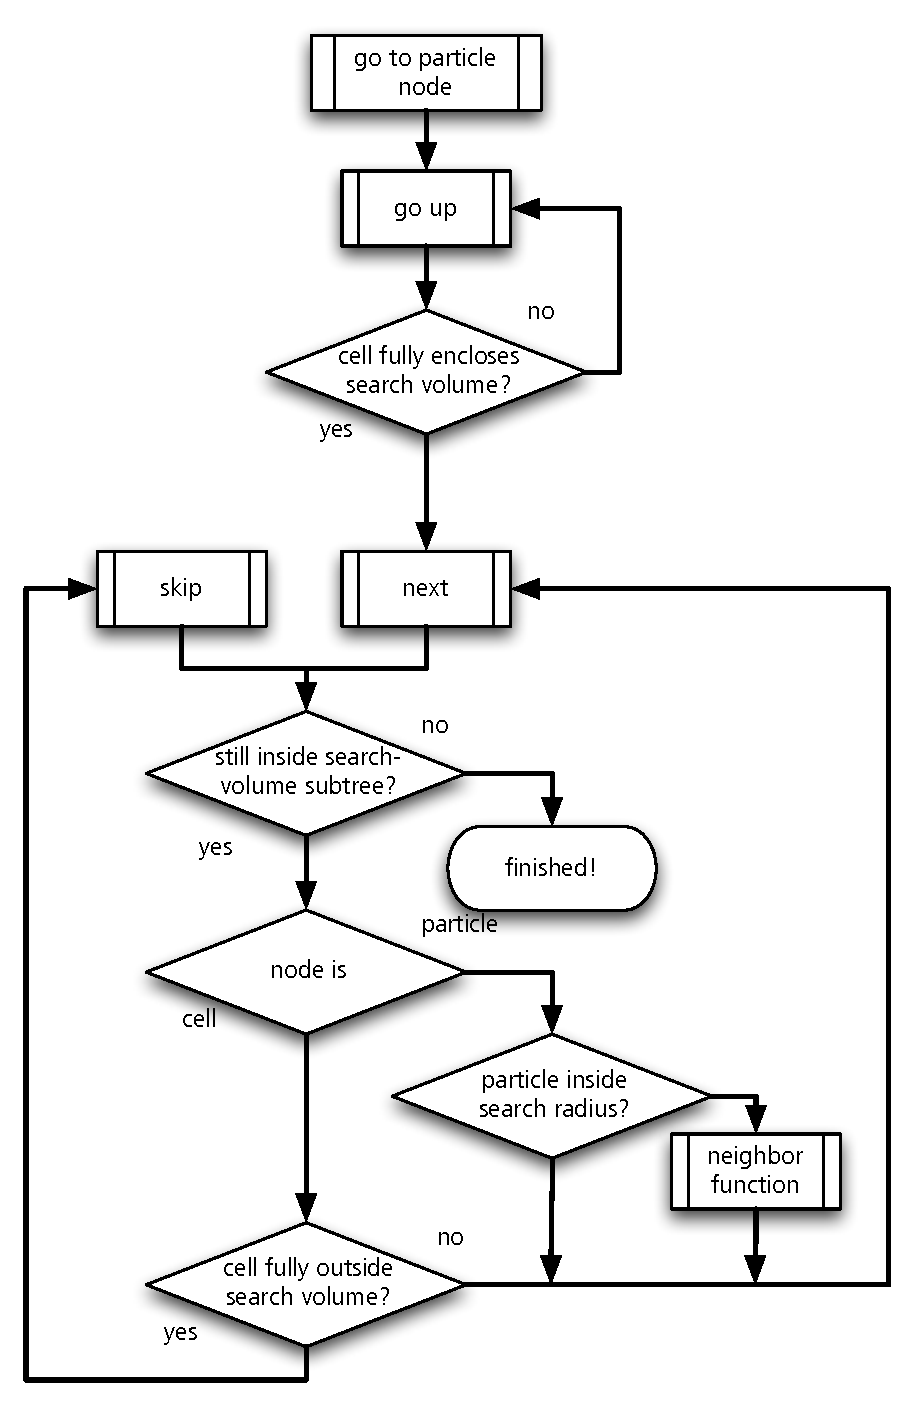
\includegraphics[scale=0.6]{16algo_neighsearch.pdf}
\caption{A non-recursive algorithm }
\label{ch02_grav02_fig10}
\end{center}
\end{figure}

The neighbor search algorithm is also used for other tasks, than searching for the SPH neighbors. It can also be used for example for friend-of-friend algorithms or the initial estimate of the smoothing length.

\section{Implementation: SPHLATCH}
In this section we will discuss the implementation of the SPH and selfgravity tree code SPHLATCH. Figure \ref{ch02_grav02_fig11} shows the basic outline of a common particle code. In a first step, the particles are loaded. Other data like tables for the equations of state are loaded as well. After that the main loop starts, which integrates the particles forward in time. Some integrators like the Predictor-Corrector scheme from equations \ref{ch02_sph02_eq019} - \ref{ch02_sph02_eq021} first determine the maximum allowed timestep. Then the derivatives are calculated several times, two times in case of the Predictor-Corrector. At certain points in time, special tasks like storing the particles or some post-processing is done. When the particles have been forwarded in time 


\begin{figure}[htbp]
\begin{center}
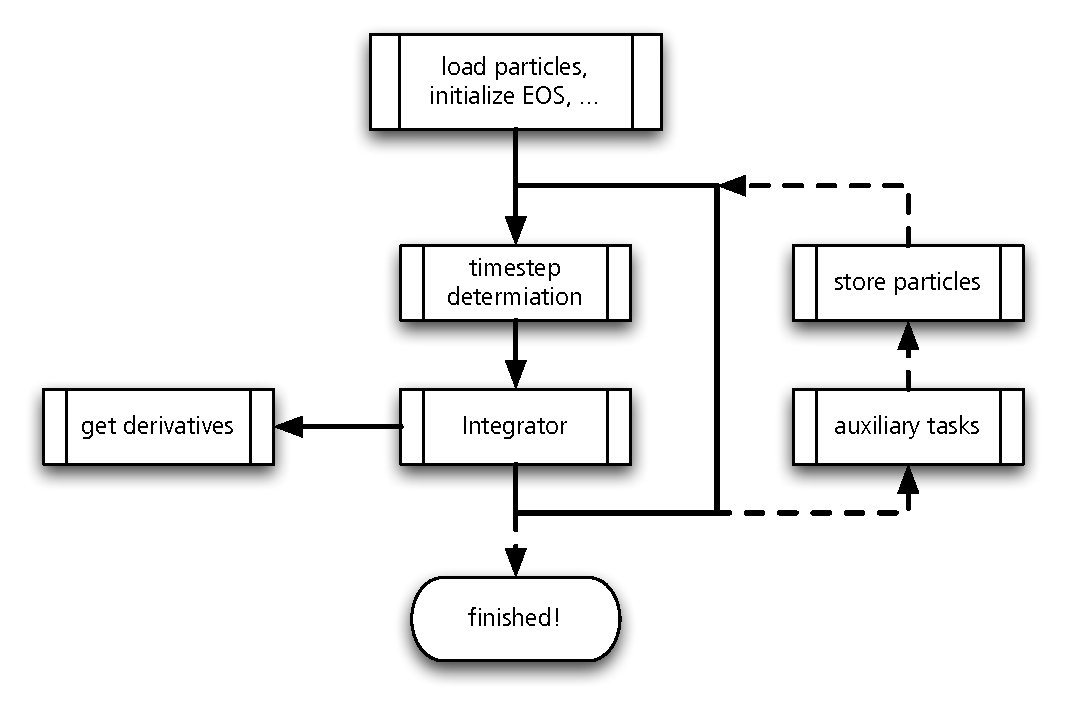
\includegraphics[scale=0.6]{20algo_overview.pdf}
\caption{Overview of the tasks in a common particle code. The main loop consists of the integrator evolving the particles forward in time. The most time consuming part of the code is the derivation step, where derivatives of integrated values are calculated.}
\label{ch02_grav02_fig11}
\end{center}
\end{figure}

\subsection{Tree and code parallelization: shared vs. distributed memory}
Since the introduction of electronic computers based on semiconductors, the transistor count on a microchip doubled every 18 months \citep{Moore:1965p4006}. Similarly also the performance, measured in FLOPS (floating point operations per second), increased over time. While up until the late 1990ies, this performance increase could be guaranteed by simply increasing the clocking frequency and complexity of the CPUs. After that physical limits upon the frequency and the size semiconductor structures capped the performance increase of a single CPU \footnote{A single CPU can be understood as a unit capable of running independently a computer program}. So the computer industry started to face this problem by simply increasing the number of CPU cores per computer. The increased performance can therefore only be harvested, if a program can run in \emph{parallel} on several CPU cores. There exist basically two types of parallelization: 
Distributed memory computing is based on several computers with independent memory, but with a common network over which they can exchange data. A popular approach in scientific computing is MPI, a software library which provides functions to exchange numerical data. Often high speed networks like Ethernet or Infiniband are used as a transport media. Although it is non-trivial to parallelize a computer code with MPI, it provides a straightforward solution to use hundreds of CPUs at the same time simply by interconnecting a large number of cheap computers with a network. The first implementation of the code SPHLATCH presented here uses MPI for parallelization. 
Shared memory computing on the other hand bases on several CPU cores sharing a common memory space. Data is simply exchanged by sharing certain parts of memory. A popularly used implementation of this approach in scientific computing is OpenMP, a simple set of compiler directives parallelizing loops and vector operations. The program runs as one process, but certain tasks are subdivided into threads, which can run on individual CPU cores. The disadvantage of this approach is, that the execution of the program is limited onto one computer. Only as much CPU cores can be used, as a single computer has. While this was a limitation a decade ago, when affordable computers did not have more than two or four CPU cores, nowadays machines offer a much larger number of cores. As of 2011, server machines with 32 or 48 CPU cores are no exception. The second implementation of SPHLATCH uses OpenMP for parallelization.

\subsection{SPHLATCH v1}
The first version of SPHLATCH uses a distributed memory parallelization by employing the MPI library. The simulation space containing the particles is spatially divided into so called \emph{cost zones}. Figure \ref{ch02_grav02_fig12} shows the same particle set as in figure \ref{ch02_grav02_fig02}. In this 2D example, the cells at depth 2 are used as cost-zone cells, resulting in a total number of 16 cost-zone cells. The particles inside a cost-zone cell now is assigned to the computational domain to which this particular cost-zone cell belongs to.


The computational cost for calculating the derivatives like acceleration due to gravity or some SPH-sum in an SPH calculation, is typically of the same magnitude for every single particle. So a natural way of parallelizing such a calculation is to divide the set of particles used in the calculation into about equally sized subsets. Each subset is then assigned to a process. 


These subsets can be created by subdividing the space in which all particles lie into \emph{computational domains}, volumes containing the desired subset of particles. These volumes are called \emph{cost-zone volumes}. For the parallelization method used for the tree, it is necessary to build these computational domains out of volumes with a side length of $l / 2^{d_{cz}}$, where $l$ is the side length of the root node of the octree or in other words the side length of the smallest cube containing all the particles aligned with the coordinate system. $d_{cz}$ is the \emph{cost zone depth}.




\begin{figure}[htbp]
\begin{center}
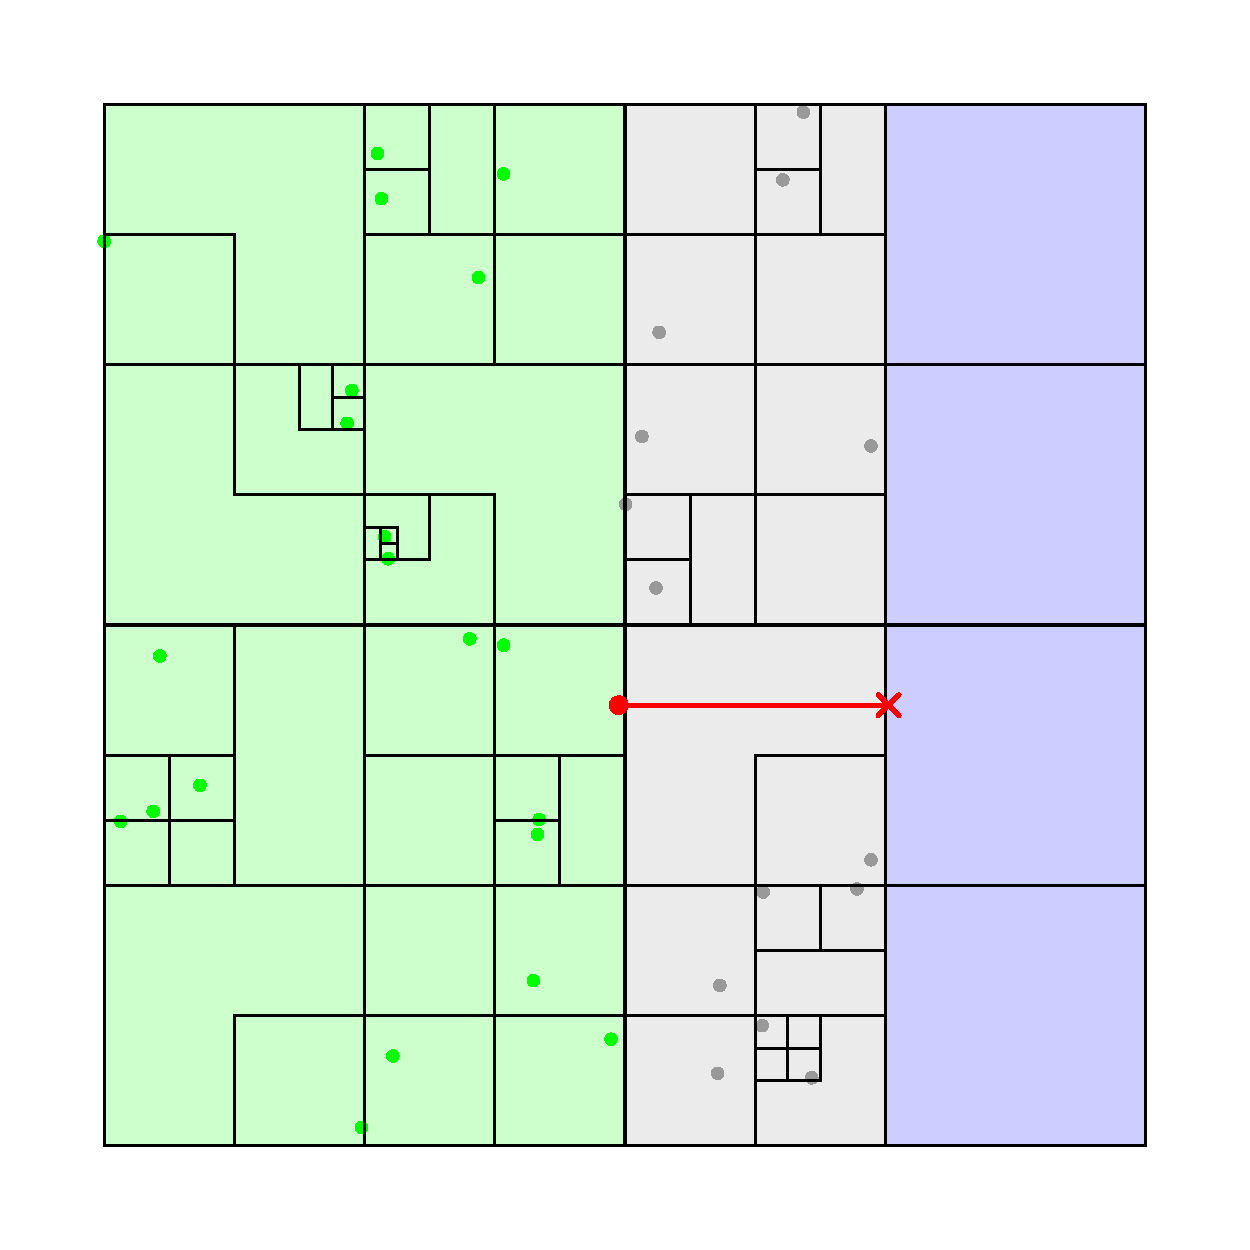
\includegraphics[scale=0.6]{07quadtree50_xy_TPL2.pdf}
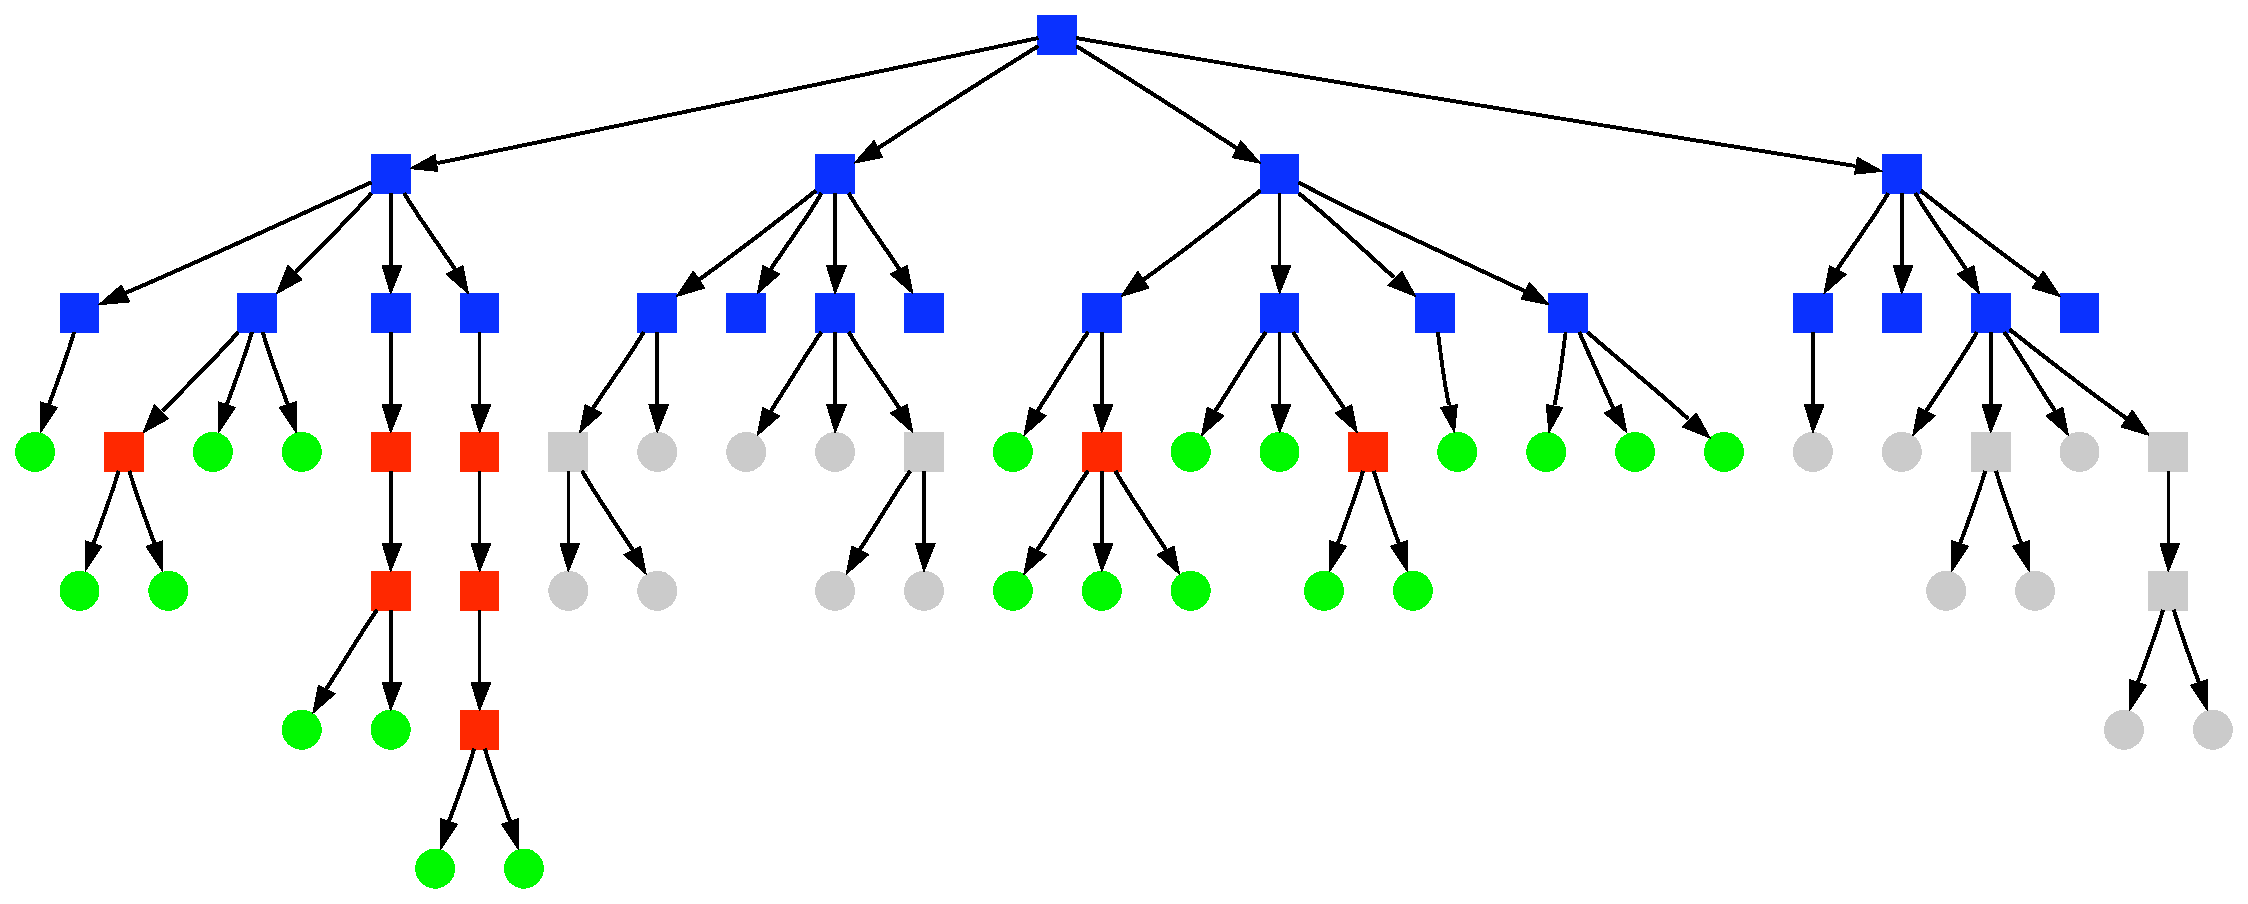
\includegraphics[scale=0.3]{07quadtree50_TPL2_stage3.pdf}
\caption{A part of the same particle distribution like in figure \ref{ch02_grav02_fig02}. The local domain is shaded green and contains 21 particles for which the acceleration has to be calculated. Bordering this zone is the ghost domain shaded grey, for which all particles are known. Beyond that, no particle information is available, only the corresponding parts of the global tree down to top-tree depth are known here. The plot below shows the corresponding tree. Note the filled top-tree nodes without any children nodes, they correspond to the domain where no particle information is available.}
\label{ch02_grav02_fig12}
\end{center}
\end{figure}

Figure \ref{fig:2D_BHtree_costzone} shows one computational domain of such a partition of the same particle distribution like in figure \ref{fig:2D_BHtree}. The $21$ particles calculated in the current computational are called \emph{local particles} and are shown in green, the corresponding cost-zone volumes are shaded green. In this example the cost-zone depth is $2$ or the cost-zone volumes are obtained by subdividing space twice in each dimension. \\

Local particles may need information about particles in other computational domains. To compute an SPH-sum for a particle, usually information about particles within two smoothing lengths is needed. When a local particle is right at the edge of the domain, it needs to know about non-local particles in the adjacent domain. Particles inside non-local volumes sharing an edge with a local volume are called \emph{ghost particles} oder just \emph{ghosts}. Besided having to be copied on to the local process, they cause no computational cost, as only their information is used but nothing is calculated for them.\\

It is desirable to have as little ghost particles as possible. The way the computational domains and subsequently are made up by combining the cost-zone volumes determine the number of ghost. Generally it is best to minimize the surface of the computational domains. Composing the domains by cutting space-filling curves like the \emph{Peano-Hilbert-walk} along the cost-zone volumes into intervals leads usually to good results.\\

Parallelizing the gravity calculation with a  B\&H-tree is not as straightforward like parallelizing a particle calculation for short-range forces, where interaction with distant non-local particles just can be omitted. The crucial point is to know, which parts the local particles need to know about the \emph{global tree} generated by all the particles, local and non-local. The tree known to the local particles is called the \emph{local tree} and provides all the necessary information to the local particles. It differs from the \emph{global tree} as such as it does not contain sub-trees not needed by the local particles. The sub-trees which can be omitted are be easily identified by the MAC and a worst-case scenario for the distribution of a local and a non-local particle shown in figure \ref{fig:2D_BHtree_costzone}. Assume a particle right at the edge of the computational domain, marked in the figure with a red dot. The shortest distance between this particle and any point in the non-local domain for which no particle information is available, marked in the figure with a red line, is the side length of the cost zone volumes or in other words the distance between the particle any point in the non-local domain $r_{WC}$ is always bigger than this side length:
\begin{equation}
r_{WC} \ge \frac{l}{2^{d_{CZ}} } 
\end{equation}
The MAC now tells us how big a cell might be to still be accepted for acceleration calculation, given the worst case distance or in other words, it tells us how deep we have to go in the tree until the multipole approximation is acceptable. Taking the worst case with distance $r_{WC}$ we get the deepest depth we have to go in the tree for a point in the non-local domain, we'll call that the \emph{top-tree depth} $d_{TT}$
\begin{equation}
\frac{l_{cell}}{r_{WC}} = \frac{l}{r_{WC} 2^{d_{TT}}} \ge \theta
\end{equation}
The top-tree depth is down to which the global tree has to be known on every computational domain. Any tree-structure below that depth is either provided by the local or ghost particles, or is not needed locally. Combining the two equations we get a relation between the top-tree depth, the costzone depth and the opening angle from the MAC:
\begin{equation}
2^{d_{CZ} - d_{TT}} \le \theta ~~~~\text{or}~~~~ d_{TT} = d_{CZ} + \uparrow \Big( - \frac{ \log{\theta} }{\log{2} } \Big)
\end{equation}
The first expression tells us down to which opening angle the local tree provides enough information for a given costzone and top tree depth. The latter expression gives the minimal needed top tree depth for a given costzone depth and opening angle. The rounding up is because depths are always integer numbers. The example shown in  figure \ref{fig:2D_BHtree_costzone} uses a top-tree depth of 2 and also a costzone depth of 2, so $\theta \ge 1$. In order to use a smaller opening angle we would have to increase the top-tree depth.\\

So we know now which parts of the global tree need to be in the local tree. The next question is how to build the local tree. On no process the global tree can be built, as no process knows about all the particles and also the global tree might be too big to fit into the memory available to a process. The basic idea is to build the local tree with local and ghost particles and then synchronize the \emph{top-tree} which is the global tree starting from the root node down to top-tree depth.

Synchronizing the top-tree is per se non-trivial, as a process does not know which parts of the non-local domain contain particles and therefore need nodes to represent them and which don't. The easiest solution is to build a \emph{full} top-tree, this means each node in the top-tree contains the maximum possible number of children. In 2D this corresponds to a full quad-tree, in 3D to a ful octree. The problem is now, that for non-uniform particle distributions we get many top-tree nodes not containing any particles in or below them, which will lead to unnecessary walks along them and vanishing contributions to the acceleration. The calculation does not get incorrect, but the adding up of vanishing terms leads to a higher computational cost. Therefore we introduce an \emph{emptiness} flag to each cell node. A priori a cell nodes is empty. Only when a particle is inserted the cell node becomes unempty or in other words filled. Emptiness is inherited bottom-up from the children to the parent node in a logically negative way, this means when a node has any non-empty child, it becomes non-empty. This flag can now be queried during tree-walks in order to avoid empty walking along empty sub-trees. So we start building the tree by setting up a full top-tree consisting of empty nodes. The first tree in figure \ref{fig:2D_BHtree_building} shows such an empty quadtree with top-tree depth of two. Every process now has a top-tree of the same structure and therefore we avoid synchronizing different tree structures between the processes.\\

During the next step, the particles locally known to a process, namely the local and ghost particles, are added to the local tree, inserting cell nodes where needed. After that the multipole moments can be calculated bottom-up from the children to their parents. This is a little bit tricky again, as a particle may be present on different process at the same time: On the process assigned to its computational domain as a local particle and to one or more domains as a ghost particle. We have to make sure, that such particles contribute to the multipole moments of the tree only once. But we also have to make sure, that the ghost particles contribute to the multipole moments of a ghost cell node. An example of such a ghost cell node can be seen in the third and fourth tree in figure \ref{fig:2D_BHtree_building} represented by grey squares. This ghost cell nodes may also be used for the acceleration calculation and therefore have to contain the correct multipole moments. For this reason we introduce a \emph{locality} flag to each node. A local particle has the locality \emph{local}, a ghost particle the locality \emph{remote}. Locality is again inherited bottom-up from the childred to their parent nodes in a positive sense. If one children is local, the parent node is also local. Only when all children are remote, the parent is remote. Top-tree nodes are excluded from this rule and have always the locality local. So when calculating the multipole moments of a node, we apply the rule that only nodes with the same locality contribute to the multipole moments. With that rule we fulfill both requirements mentioned above: Ghost cell and particle nodes do not contribute to the globally synchronized top-tree, but ghost cell nodes still get their correct multipole moments based on their remote or ghost children.\\

After adding up the multipoles, we can sum up the multipole moments of the top-tree. This is straightforward, as all top-trees have the same structure. The emptiness flag is summed up using an OR-relation, respecting the additive nature of multipole moments addition. After this step we end up with a valid Barnes\& Hut tree containing all the required particles and cells needed to calculate the gravitational acceleration for the local particles.\\

This parallelization method is rather simple, which is one of the advantages of it. Another advantage is, that after the particles and ghosts have been copied to the processes, only one, big additional communication step is required for summing up the multipole moments of the top-tree nodes. When summing up the multipole moments between two processes, all the data can be sent to one process and summed up there. This is bulk communication and therefore ideal for communication networks with high bandwidth. Latency is not important. In practice, the synchronization needs only a few percent of the total time of the gravity calculation using a reasonably fast network.\\

The downside of the method is that for non-uniform particle distribution a lot of unused and empty top-tree nodes have to be created. Although they don't need to be accessed, they use memory and worsen the caching of other tree nodes. The enforcement of cell nodes in the top-tree also causes a deeper tree than without the top-tree, which lead to longer and thereforce slightly slower tree walks.\\



\begin{figure}[htbp]
\begin{center}
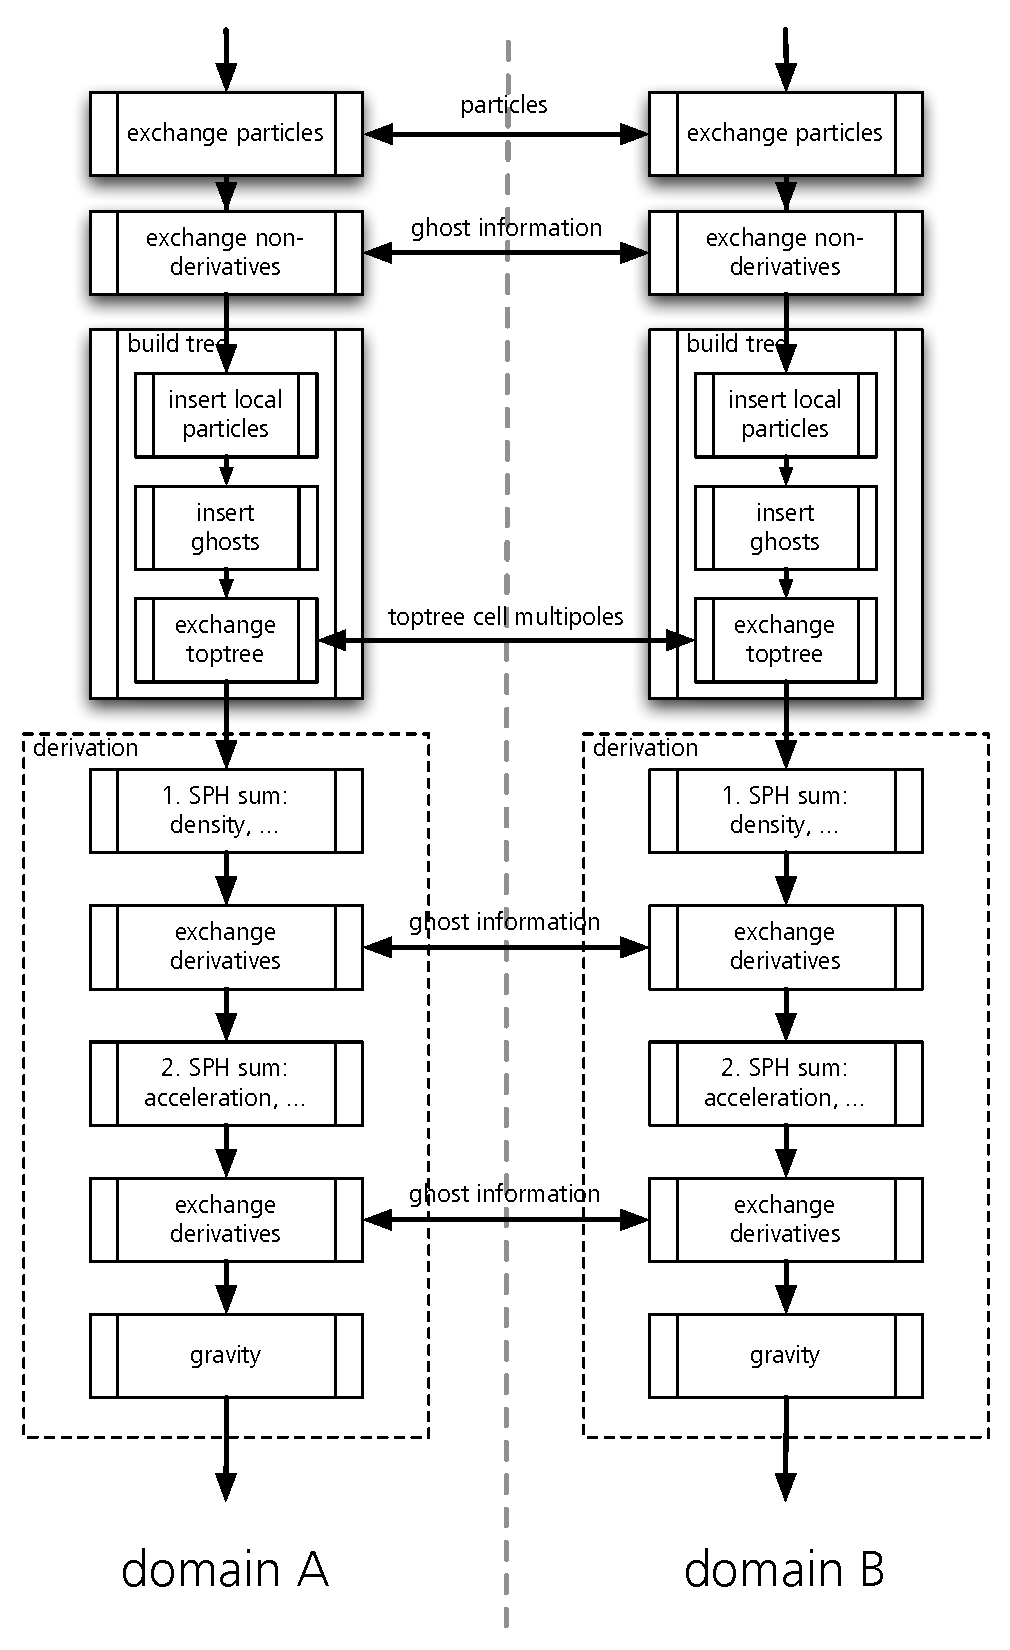
\includegraphics[scale=0.6]{21algo_sphlatch01.pdf}
\caption{Overview of the derivation step for SPHLATCH v1. }
\label{ch02_grav02_fig12}
\end{center}
\end{figure}


SPHLATCH v1\\
parallelizing a particle code: distributed sums vs. ghosts approach\\
parallelizing a tree\\
show ghost approach\\
disadvantage of a simply spatial decomposition\\
% TODO: show actual cost in GI simulations

disadvantage: distributed memory machines loose importance, not good for parameter space searches, mutlicore machines are the future


% TODO: number of pointers, memory requirements
% TODO: show two flow diagrams of both codes: derivatiion, integration, loading, auxiliary




\begin{figure}[htbp]
\begin{center}
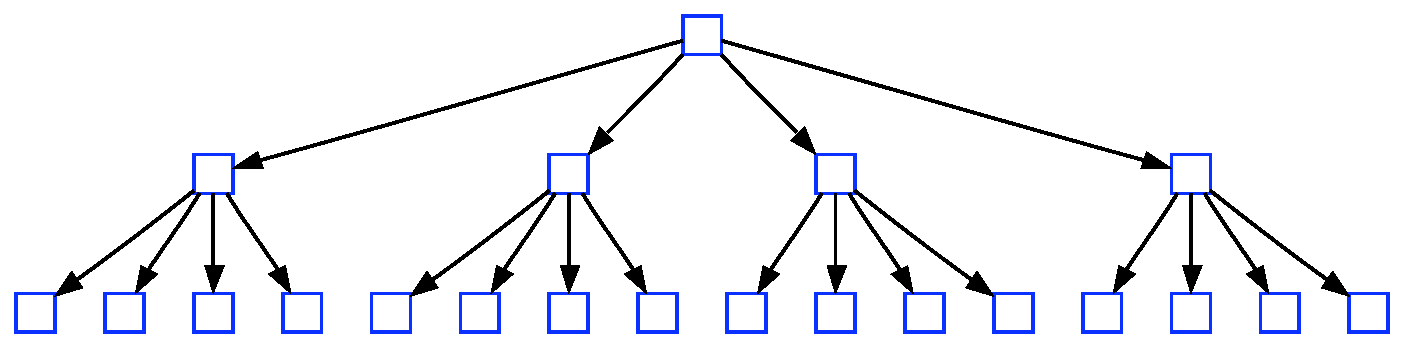
\includegraphics[scale=0.35]{07quadtree50_TPL2_stage1.pdf}\\ \vspace{1.0cm}
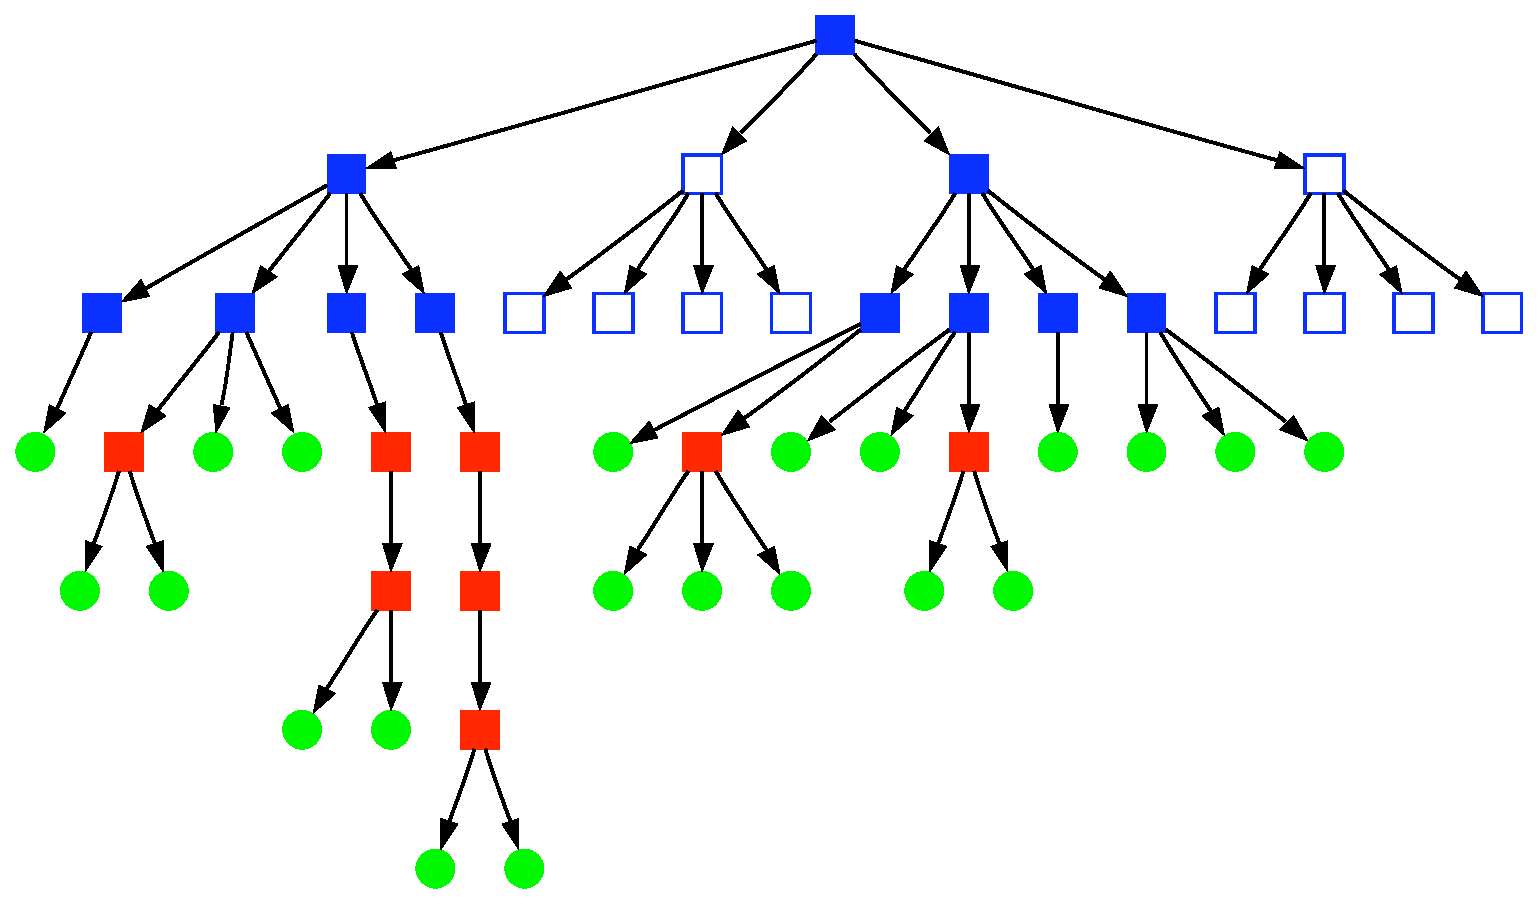
\includegraphics[scale=0.35]{07quadtree50_TPL2_stage2a.pdf}\\
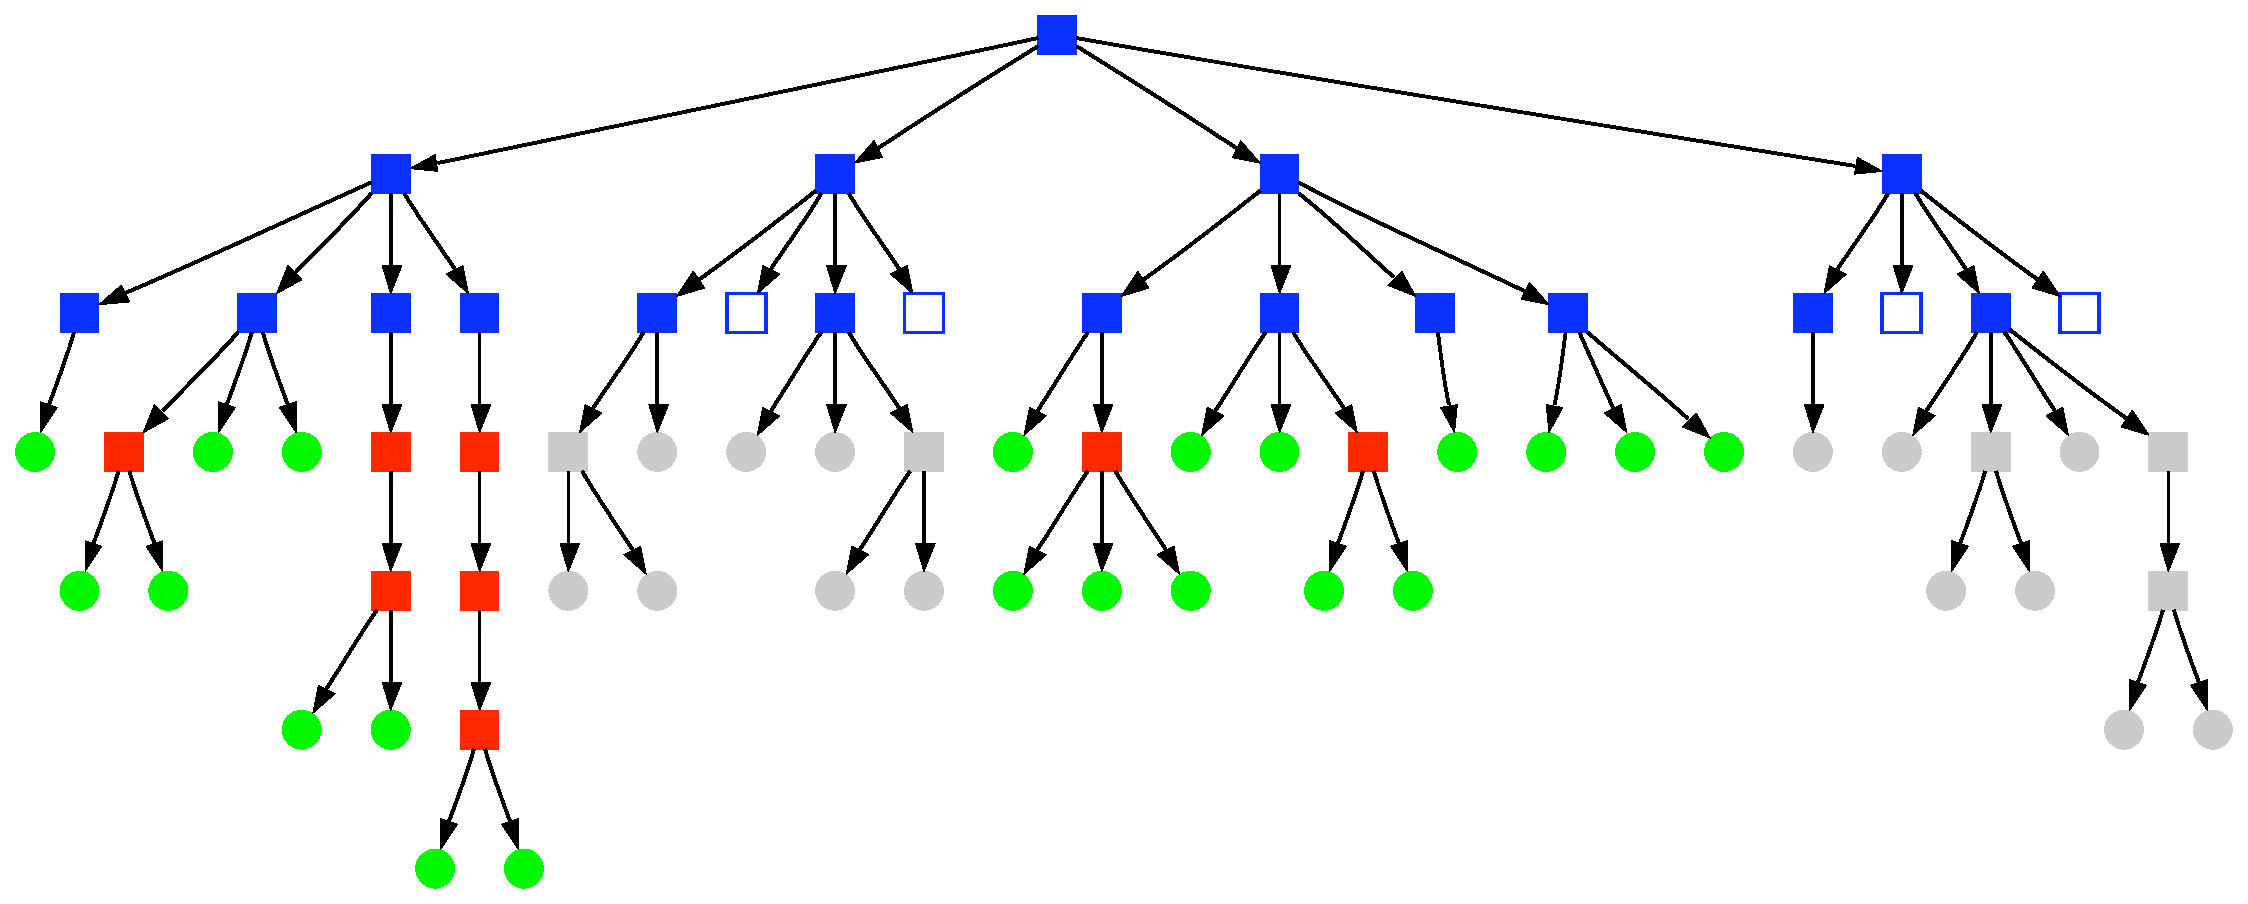
\includegraphics[scale=0.35]{07quadtree50_TPL2_stage2b.pdf}\\
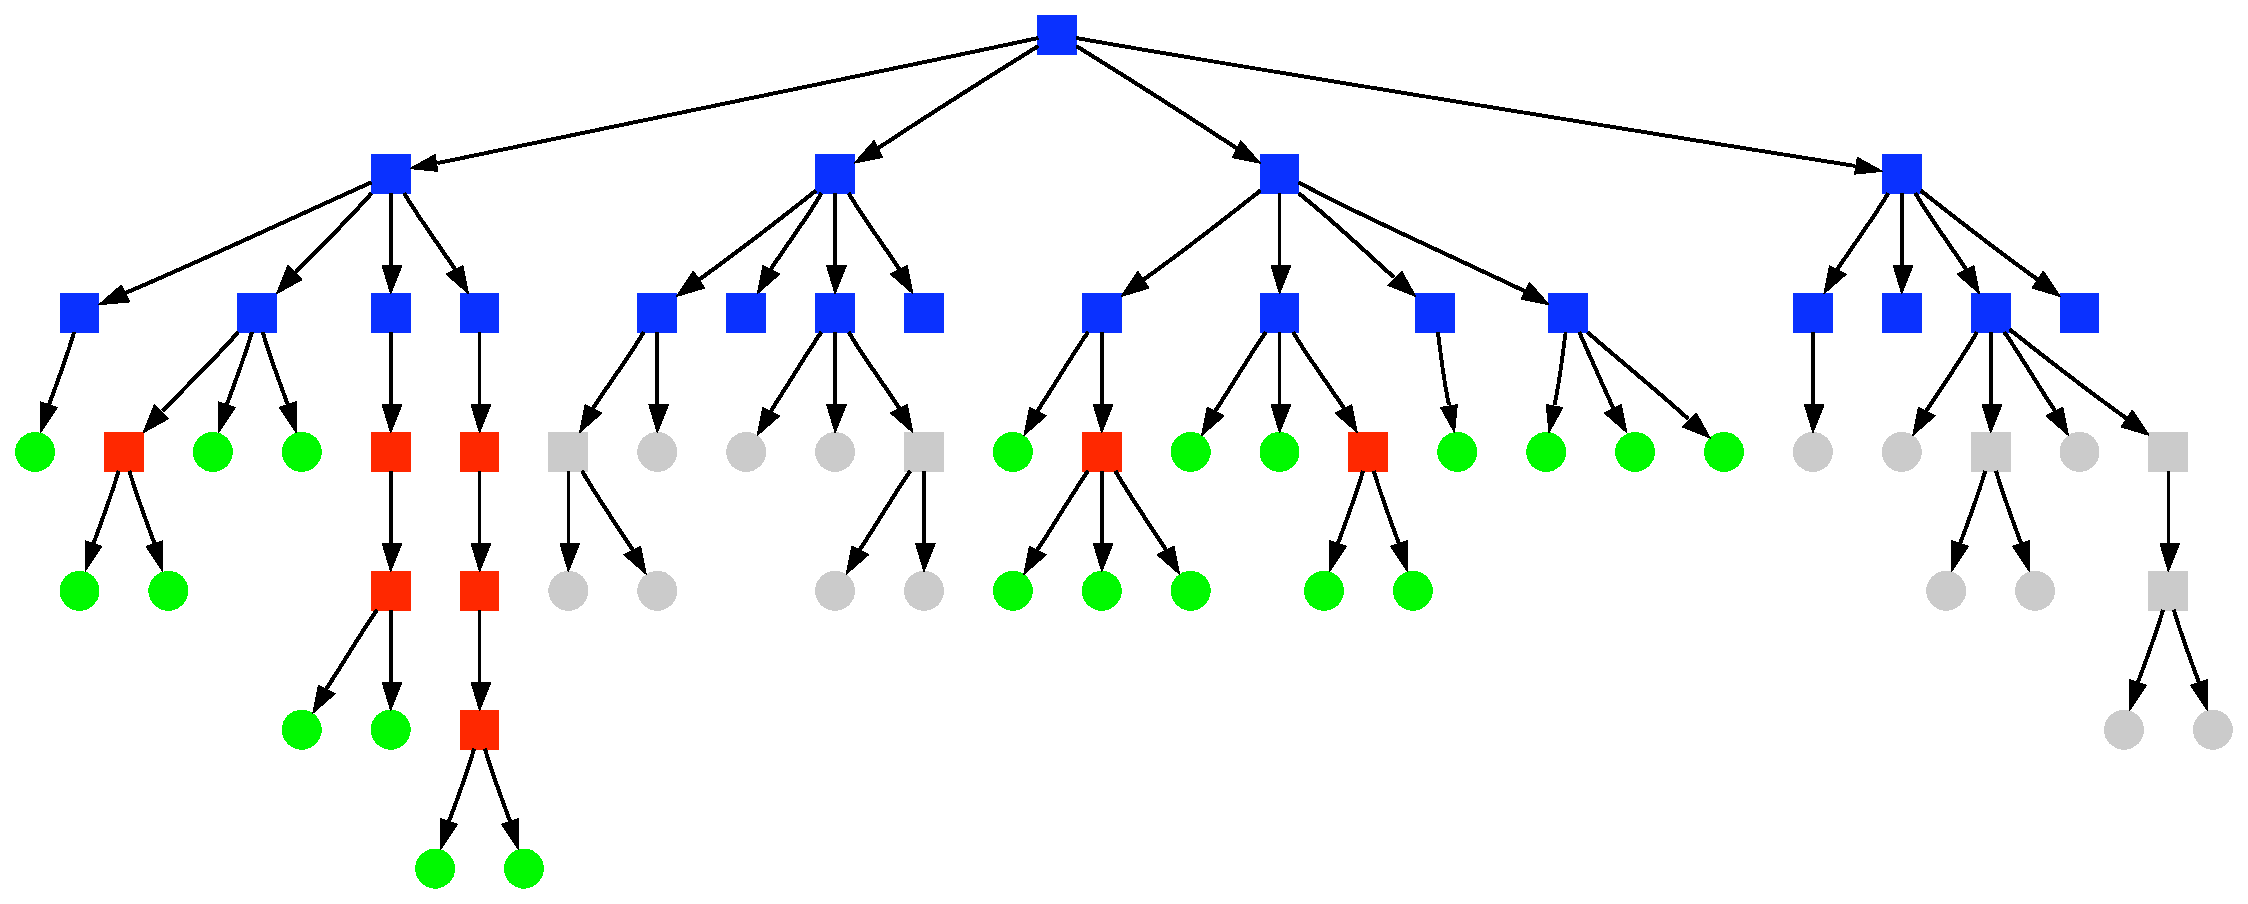
\includegraphics[scale=0.35]{07quadtree50_TPL2_stage3.pdf}\\
\caption{Building stages of the local tree for the computational domain in figure \ref{fig:2D_BHtree_costzone}. The first tree shows the empty top-tree, a full quad-tree with depth 2. Then the local and the ghost particles are inserted leading to the second and third tree. As a final step the top-tree is summed up globally, filling up the 4 previously empty cell nodes. Top-tree cell nodes are coloured blue, normal cell nodes red and particles green. Ghost particles or cells are coloured grey. Non-filled shapes represent empty nodes.}
\label{fig:2D_BHtree_building}
\end{center}
\end{figure}




\subsection{SPHLATCH v2}

\begin{figure}[htbp]
\begin{center}
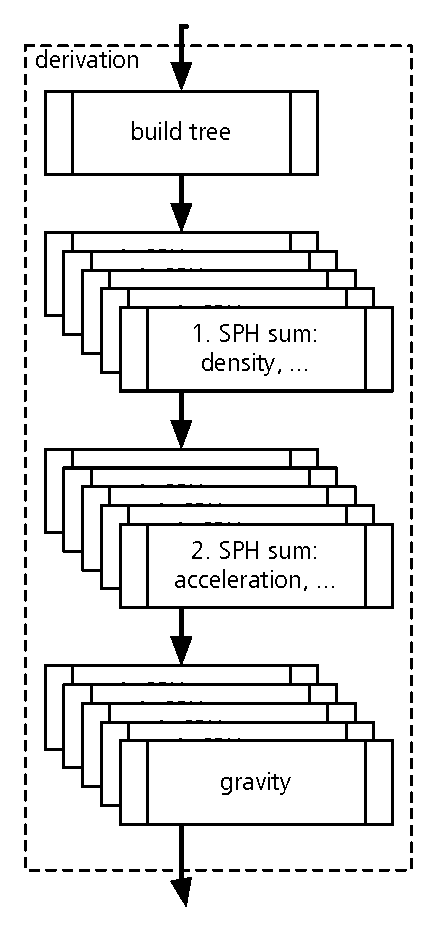
\includegraphics[scale=0.6]{22algo_sphlatch02.pdf}
\caption{}
\label{ch02_grav02_fig12}
\end{center}
\end{figure}


SPHLATCH v2\\
shared memory approach\\
load balancing approach, how this could be memory-\\
show cost (gravity, NS, total) for giant impact\\
caching issues\\

building the tree:



\subsection{Future of particle codes}
mention future of parallel computing: CPU vs. GPU computing, stream computing
trees on GPUs (references)



\section{Initial conditions}
\subsection{vanilla SPH sphere}
\subsection{getting 1D structures}
\citep{Benz:1991p700}

\subsection{flavouring an SPH sphere}
\subsection{putting an atmosphere on top}
initial conditions: show theoretical vs. unevolved vs. evolved densities, show example of impact with standard SPH and miscible SPH (chondritic, use moon case), setting up a \SSC \\
use of spheres for simplicity reason


\section{Post-processing}
\subsection{clump detection}
\subsection{plotting}
clump detection\\
FOF vs. potential, not parallelized\\

\section{Tests}
shocktube
simple gravity tree

\citep{Abel:2010p3297}
\citep{Barnes:1986p2853}
\citep{bryant2010computer}
\citep{Melosh:2007p3502}
\citep{Monaghan:2005p2677}
\citep{Monaghan:1992ARAA..30..543M}
\citep{Ott:2003p3727}
\citep{Price:2004p2613}
\citep{Solenthaler:2008p3720}
\citep{Springel:2003p3298}
\citep{Springel:2005p51}



\bibliographystyle{plainnat}
\bibliography{bibliography}


